% =====================================================================
%  PyPRIMAT — extensive user + physics documentation
%
%  Figures are produced by the companion notebook in this folder,
%      doc/PyPRIMAT_doc_figures.ipynb
%  which writes PDF figures into doc/figures/.  Re-run that notebook
%  (Kernel -> Restart & Run All) before recompiling this document if the
%  code has changed.
%
%  Compile with:   latexmk -pdf PyPRIMAT_documentation.tex
%             or:  pdflatex PyPRIMAT_documentation.tex  (x3 for refs)
% =====================================================================
\documentclass[11pt,a4paper]{article}

\usepackage[utf8]{inputenc}
\usepackage[T1]{fontenc}
\usepackage{lmodern}
\usepackage[margin=2.4cm]{geometry}
\usepackage{amsmath,amssymb}
\usepackage{graphicx}
\usepackage{booktabs}
\usepackage{longtable}
\usepackage{array}
\usepackage{xcolor}
\usepackage{listings}
\usepackage{caption}
\usepackage[colorlinks=true,linkcolor=blue!55!black,citecolor=green!45!black,%
            urlcolor=blue!55!black]{hyperref}

\graphicspath{{figures/}}

% Allow the justification engine a little extra slack so long unbreakable
% monospace identifiers (e.g. compute_detailed_balance_coefficients) do not
% produce overfull lines in running text.
\setlength{\emergencystretch}{5em}

% ----- code-listing style ------------------------------------------------
\definecolor{codebg}{rgb}{0.97,0.97,0.95}
\definecolor{codekw}{rgb}{0.10,0.10,0.65}
\definecolor{codecm}{rgb}{0.30,0.50,0.30}
\definecolor{codestr}{rgb}{0.60,0.20,0.20}
\lstdefinestyle{shared}{
  backgroundcolor=\color{codebg},
  basicstyle=\ttfamily\small,
  keywordstyle=\color{codekw}\bfseries,
  commentstyle=\color{codecm}\itshape,
  stringstyle=\color{codestr},
  showstringspaces=false,
  breaklines=true,
  frame=single,
  rulecolor=\color{black!20},
  framesep=4pt,
  columns=fullflexible,
  numbers=none,
}
\lstdefinestyle{py}{style=shared,language=Python}
\lstdefinestyle{sh}{style=shared,language=bash}
\lstset{style=shared}

% ----- handy physics macros ----------------------------------------------
\newcommand{\dd}{\mathrm{d}}
\newcommand{\ii}{\mathrm{i}}
\newcommand{\Tg}{T_\gamma}
\newcommand{\Tnu}{T_\nu}
\newcommand{\Neff}{N_{\mathrm{eff}}}
\newcommand{\YP}{Y_P}
\newcommand{\DoH}{\mathrm{D/H}}
\newcommand{\sigmav}{\langle\sigma v\rangle}
\newcommand{\code}[1]{\texttt{#1}}
\newcommand{\PR}{Phys.\ Rep.}
\newcommand{\Gap}{\Delta}
\newcommand{\Kw}{\mathcal{K}}
\newcommand{\NA}{N_A}
\newcommand{\afs}{\alpha_{\mathrm{FS}}}
\newcommand{\cLL}{c_{LL}}
\newcommand{\cRR}{c_{RR}}
\newcommand{\cLR}{c_{LR}}

\title{\textbf{PyPRIMAT}\\[2pt]
       \large A Python package for precision Big Bang Nucleosynthesis\\[6pt]
       \normalsize User guide and physics reference}
\author{Cyril Pitrou}
\date{\today}

\begin{document}
\maketitle

\begin{abstract}
\noindent
PyPRIMAT is a Python re-implementation of the \code{PRIMAT} code for precise
Big Bang Nucleosynthesis (BBN). It integrates the coupled equations governing
(i) the cosmological background -- photon and neutrino temperatures and the
scale factor -- and (ii) a nuclear reaction network, to predict the primordial
abundances of $^{1}$H, D, $^{3}$He, $^{4}$He, $^{7}$Li and heavier nuclides.
This document is meant to be \emph{self-contained}: the main text shows how to
\emph{use} the code (Sec.~\ref{sec:usage}) and gives the working equations for
the three physical ingredients -- the plasma thermodynamics
(Sec.~\ref{sec:plasma}), the $n\leftrightarrow p$ weak interactions
(Sec.~\ref{sec:weak}) and the thermonuclear network (Sec.~\ref{sec:nuclear}) --
together with the run-time options that control them, followed by a section on
the sensitivity of the abundances to the inputs (Sec.~\ref{sec:sensitivity}).
All the lengthy formulas needed to actually reproduce the code -- the full QED
plasma corrections, every correction to the weak rates beyond the Born
approximation, and the detailed-balance/NSE derivation -- are collected in the
appendices, so that the algorithms can be rewritten from this document alone.
Equations follow the review of Pitrou, Coc, Uzan \& Vangioni,
\emph{Physics Reports} \textbf{754} (2018) 1 \cite{PhysRep2018} (cited as
``\PR''), and references therein, which the reader should consult for
derivations.  Figures are produced by the companion notebook
\code{PyPRIMAT\_doc\_figures.ipynb}.
\end{abstract}

\tableofcontents

% =====================================================================
\section{Quick overview: using the code}\label{sec:usage}
% =====================================================================

PyPRIMAT can be driven in three equivalent ways, all of which build a parameter
dictionary and call the top-level driver \code{pyprimat.PyPR}. Run from the
repository root so that the data files under \code{rates/} resolve.

\subsection{Command-line interface}
The \code{pyprimat} console script exposes the most commonly varied options:
\begin{lstlisting}[style=sh]
pyprimat --Omegabh2 0.02242 --network medium
\end{lstlisting}
which prints a short summary:
\begin{lstlisting}[style=sh]
Neff     = 3.04397730
YP (BBN) = 0.24691155
YP (CMB) = 0.24558556
D/H      = 2.4381479e-05
He3/H    = 1.0387101e-05
Li7/H    = 5.489582e-10
--- running time: 1.22 seconds ---
\end{lstlisting}
The main flags are \code{-{}-Omegabh2}, \code{-{}-DeltaNeff}, \code{-{}-network}
(\code{small}/\code{medium}/\code{large} or any custom network file),
\code{-{}-amax}, \code{-{}-numerical\_precision}, \code{-{}-json} (dump the full
result dictionary), and \code{-{}-verbose}.

\subsection{Python API}
For full control, build a parameter dictionary and call \code{PyPR} directly;
every key of \code{config.DEFAULT\_PARAMS} is accepted.
\begin{lstlisting}[style=py]
from pyprimat import PyPR

result = PyPR({"Omegabh2": 0.022425, "network": "medium"}).solve()
print(f"YP  (BBN) = {result['YPBBN']:.8f}")   # 0.24700173
print(f"D/H       = {result['DoH']:.7e}")      # 2.4356100e-05
print(f"Neff      = {result['Neff']:.8f}")     # 3.04397730
\end{lstlisting}
The \code{solve()} call returns a dictionary with \code{Neff}, the helium mass
fractions \code{YPBBN}/\code{YPCMB}, the ratios \code{DoH}, \code{He3oH},
\code{He3oHe4}, \code{Li7oH}, and the neutrino observables
\code{Omeganurel}/\code{OneOverOmeganunr}. The \code{PyPR} instance also exposes
the background history and abundance trajectories as attributes used throughout
the companion notebook: the temperature vectors \code{\_Tg\_vec},
\code{\_Tnue\_vec}, the weak-rate interpolants \code{\_nTOp\_frwrd},
\code{\_nTOp\_bkwrd} (functions of $\Tg$ in \emph{kelvin}), the compiled forward
reaction rates \code{nucl.<reaction>\_frwrd} (function of $T$ in kelvin,
internally $T_9=T/10^9$), the abundance interpolant \code{\_Y\_of\_t}, and the
final values \code{\_Y\_final}.

\paragraph{Output files.}
\code{output\_time\_evolution=True} writes \code{results/output\_tables.tsv}
with the full background and per-nuclide history; \code{output\_final\_result=True}
writes the final mass fractions.

\subsection{Graphical interface}
After \code{pip install -e ".[gui]"}, a browser-based Streamlit app is available:
\begin{lstlisting}[style=sh]
pyprimat-gui                       # console-script launcher
streamlit run pyprimat/gui/app.py  # from a source checkout
\end{lstlisting}
It exposes the parameters as form fields and shows the final abundances and an
interactive abundance-evolution plot.

\subsection{Reading the numerical output}
Several physical corrections shift $\Neff$ at the $10^{-2}$--$10^{-3}$ level, so
abundances should be reported with enough significant figures: at least 8
decimals for $\Neff$ and $\YP$, 7 for $\DoH$, and 6 for $^{7}$Li/H. A standard
small-network run with $\Omega_b h^2 = 0.022425$ gives $\YP \simeq 0.24700$,
$\DoH \simeq 2.4349\times10^{-5}$ and $\Neff \simeq 3.04398$.

% =====================================================================
\section{Plasma thermodynamics}\label{sec:plasma}
% =====================================================================

\subsection{Background equations}
The BBN background is a hot plasma of photons, electrons/positrons and three
neutrino species in a spatially-flat Friedmann--Lema\^itre spacetime. Each
species is described by a distribution function $f(t,p)$ obeying the Boltzmann
equation in an expanding universe (\PR\ Eq.~12),
\begin{equation}
  \frac{\partial f}{\partial t} - H\,p\,\frac{\partial f}{\partial p}
  = C[f],
\end{equation}
whose velocity moments give the conservation laws for number density and energy
density (\PR\ Eqs.~13, 16),
\begin{equation}
  \dot n + 3 H n = \mathcal{J}, \qquad
  \dot\rho + 3H(\rho+P) = \dot q,
\label{eq:cons}
\end{equation}
with $\mathcal{J}$ and $\dot q$ the collisional source terms. The thermodynamic
quantities are momentum integrals of $f$; for a species of degeneracy $g$ and
mass $m$, writing $x\equiv m/T$, they reduce to the Fermi--Dirac ($+$) /
Bose--Einstein ($-$) integrals $I^{(n,m)}_\pm$ defined in
App.~\ref{app:thermo} (\PR\ App.~A):
\begin{equation}
  \rho = \frac{g\,T^4}{2\pi^2}\, I^{(2,1)}_\pm(x), \qquad
  P    = \frac{g\,T^4}{6\pi^2}\, I^{(0,3)}_\pm(x), \qquad
  s    = \frac{\rho+P}{T}.
\label{eq:thermo}
\end{equation}
The photon gas ($g=2$, $m=0$) has $\rho_\gamma = (\pi^2/15)\,\Tg^4$. The
expansion rate is fixed by the Friedmann equation (\PR\ Eq.~9),
\begin{equation}
  H^2 = \frac{8\pi G}{3}\,\rho_{\rm tot},
  \qquad
  \rho_{\rm tot} = \rho_\gamma + \rho_{e^\pm} + \sum_\nu \rho_\nu
                   + \delta\rho_{\rm QED} + \dots,
\label{eq:friedmann}
\end{equation}
and the scale factor $a(\Tg)$ follows from conservation of the comoving
electromagnetic-plasma entropy $\mathcal{S}\,a^3$ (\PR\ Eqs.~21--24).

\subsection{Solving the background: the two ODEs $a(\Tg)$ and $t(a)$}
\label{sec:bckg-ode}
The code reduces the background to two ordinary differential equations, solved
once at start-up (\code{PyPR.\_setup\_background\_and\_cosmo}).

\paragraph{Scale factor from entropy conservation.}
Define the reduced plasma entropy $\mathcal{S}(T)\equiv\bar s_{\rm pl}/\bar
s_\gamma$ (with $\bar s_\gamma=2\pi^2/45$, so $s_{\rm pl}=\bar s_\gamma T^3
\mathcal{S}$); from Eq.~\eqref{eq:thermo}, $\mathcal{S}=1+\frac{2}{\pi^2\bar
s_\gamma}[\tfrac13 I^{(0,3)}_+(x)+I^{(2,1)}_+(x)]$, running from $11/4$ at $T\gg
m_e$ to $1$ at $T\ll m_e$ (\PR\ Eq.~28). Exact entropy conservation gives the
algebraic relation $a(T)=a_0T_0/(T\,\mathcal{S}^{1/3})$ (\PR\ Eq.~29). With
incomplete neutrino decoupling the plasma loses entropy to the neutrinos at a
dimensionless heating rate $\mathcal{N}(T)$ defined by $\dot q_{\rm pl}/(HT)=
-T^3\mathcal{N}$ (\PR\ Eq.~57), and the relation becomes the ODE actually
integrated (\PR\ Eq.~58),
\begin{equation}
  \frac{\dd\ln a}{\dd\ln T}
  = -\,\frac{3\,\bar s_{\rm pl}+T\,\dd\bar s_{\rm pl}/\dd T}
            {\mathcal{N}+3\,\bar s_{\rm pl}},
  \qquad \bar s_{\rm pl}\equiv \frac{s_{\rm pl}(T)}{T^3},
\label{eq:aofT}
\end{equation}
which reduces to $a\propto(T\mathcal{S}^{1/3})^{-1}$ when $\mathcal{N}=0$ (the
QED-corrected $\mathcal{S}^{\rm QED}$ of App.~\ref{app:qed} is used when QED is
on). In the code $\bar s_{\rm pl}$ and $\dd\bar s_{\rm pl}/\dd T$ are returned
together by \code{plasma.spl\_and\_dspl\_dT}; Eq.~\eqref{eq:aofT} is
\code{\_dlnadlnT\_NEVO}, integrated from $T_{\rm end}$ to $T_{\rm start}$ with
\code{solve\_ivp(method='LSODA')}, and inverted to $T(a)$. When
\code{external\_background=True}, $a(T)$ is instead read directly from the NEVO
table's column $x\propto a$.

\paragraph{Time from the Friedmann equation.}
With $a(T)$ -- hence $\rho_{\rm tot}(T(a))$ -- known, the Friedmann
equation~\eqref{eq:friedmann} is integrated as
\begin{equation}
  \frac{\dd t}{\dd\ln a}=\frac{1}{H(a)},
  \qquad t_{\rm ini}=\frac{1}{2H_{\rm ini}}
\end{equation}
(radiation-domination start), giving $t(a)$ and its inverse by interpolation
(\code{\_dtdlna}). All subsequent eras use the resulting $T(t)$, $a(t)$,
$t(T)$. The plasma energy density entering $H$ is
$\rho_{\rm pl}=\mathcal{E}(T)\bar\rho_\gamma T^4$ with
$\mathcal{E}=1+\tfrac{30}{\pi^4}I^{(2,1)}_+(x)$ (plus the QED term
$\delta g_\rho/2$), and the three neutrino flavours contribute
$\rho_\nu=\bar\rho_\nu T_\nu^4$ each (\PR\ Eqs.~30--31).

\paragraph{Baryon density and $\eta_b$.}
Baryons are cold, $\rho_b\propto a^{-3}$, so $n_b(a)=n_{b,0}/a^3$ with
$n_{b,0}=\eta_b\,n_{\gamma,0}$ and the baryon-to-photon ratio
$\eta_b=(\Omega_bh^2)\times C_\eta$, where the conversion factor
$C_\eta=\rho^{\rm crit}_{100}/(n_{\gamma,0}m_b)$
(\code{cfg.Omegabh2\_to\_eta0b}); numerically $\eta_b\simeq6.09\times10^{-10}
(\Omega_bh^2/0.02225)$ (\PR\ Eqs.~33--35). This $n_b(a)$ sets the two-body
fluxes $\Gamma=n_b\sigmav$ of Sec.~\ref{sec:nuclear}.

\paragraph{Optional energy-density components.}
Any extra contribution to $\rho_{\rm tot}$ in Eq.~\eqref{eq:friedmann} enters
through the \code{extra\_rho} hook of \code{PyPR} (a list of functions
$\rho(\Tg)\,[\mathrm{MeV}^4]$). Two are built in: a constant extra radiation
density from $\Delta\Neff$ decoupled species (\code{plasma.rho\_nu\_extra},
$\rho=\tfrac78\,\tfrac{\pi^2}{15}\Tnu^4\,\Delta\Neff$), and Early Dark Energy
(\code{fEDE}, \code{zcEDE}, \code{wnEDE}; \code{PyPR.\_setup\_EDE}) -- a fluid
peaking at redshift \code{zcEDE} with energy fraction \code{fEDE} and
equation-of-state index \code{wnEDE}. Both modify only $H(\Tg)$, hence the
time--temperature relation.

\subsection{Neutrino decoupling and $\Neff$}
Neutrinos decouple just before $e^+e^-$ annihilation. In the idealized
\emph{instantaneous} limit, entropy conservation gives the asymptotic ratio
$\Tnu/\Tg \to (4/11)^{1/3}\simeq 0.7138$, and the radiation density is
parameterised by the effective number of neutrinos (\PR\ Eq.~62),
\begin{equation}
  \rho_{\rm rad} = \rho_\gamma\!\left[\,1
    + \frac{7}{8}\left(\frac{4}{11}\right)^{4/3}\Neff\right].
\label{eq:neff}
\end{equation}
In reality decoupling is \emph{not} instantaneous: the highest-energy neutrinos
are still coupled during annihilation and absorb a little of the released
entropy, raising $\Neff$ above 3. PyPRIMAT reads the precomputed
non-instantaneous history $\{\Tnu^{(e,\mu,\tau)}(\Tg)\}$ from a NEVO table rather
than recomputing the momentum-dependent Boltzmann hierarchy. Together with the
QED plasma corrections (below) this gives the Standard-Model value
$\Neff\simeq 3.044$ (Fig.~\ref{fig:decoupling}).

\subsection{QED plasma corrections}
Electromagnetic interactions between the $e^\pm$ and the photon bath shift the
effective electron and photon masses and hence the plasma equation of state
(\PR\ \S II.E). To leading orders in the coupling the interaction-pressure
correction is $\delta P = \delta P_{\rm d}+\delta P_{\rm s}$, with a dominant
$O(\alpha)$ term and a subdominant two-loop exchange term; the explicit
integrals (\PR\ Eqs.~47--49) are given in App.~\ref{app:qed}. The energy-density
correction follows from the thermodynamic identity $\rho = -P+T\,\dd P/\dd T$,
and the high-temperature limit is the constant
\begin{equation}
  \delta g_\rho \simeq \delta g_P \simeq -\frac{25\,\afs}{4\pi}\simeq -0.0145
\end{equation}
(\PR\ Eq.~52). These corrections enter in four places (App.~\ref{app:qed}): the
plasma entropy $\mathcal{S}$ that sets $a(\Tg)$, the neutrino-temperature
normalisation $z_0$, the plasma energy density in Eq.~\eqref{eq:friedmann}, and
-- through the electron mass shift, which is bookkept as a finite-temperature
weak-rate correction (App.~\ref{app:weak}) -- the weak rates.

\subsection{In the code, with figures}
Photon and neutrino thermodynamics are pure functions of temperature
(\code{plasma.rho\_g}, \code{plasma.rho\_nu}); the $e^\pm$ quantities
(\code{rho\_e}, \code{p\_e}) require the Fermi--Dirac integrals of
Eq.~\eqref{eq:thermo} and are tabulated in an electron-thermo cache. The
non-instantaneous $\Tnu(\Tg)$ history is read by \code{neutrino\_history.py};
the QED corrections are loaded from \code{rates/plasma/QED\_*.txt} or computed
analytically by \code{qed\_pressure.py}; the Friedmann rate is assembled in
\code{PyPR.\_Hubble}. Figure~\ref{fig:decoupling} shows the per-flavour
temperature ratios, Fig.~\ref{fig:gstar} the effective relativistic degrees of
freedom $g_{*\rho},g_{*s}$ through annihilation, and Fig.~\ref{fig:qed} the QED
pressure correction.

\begin{figure}[ht]
  \centering
  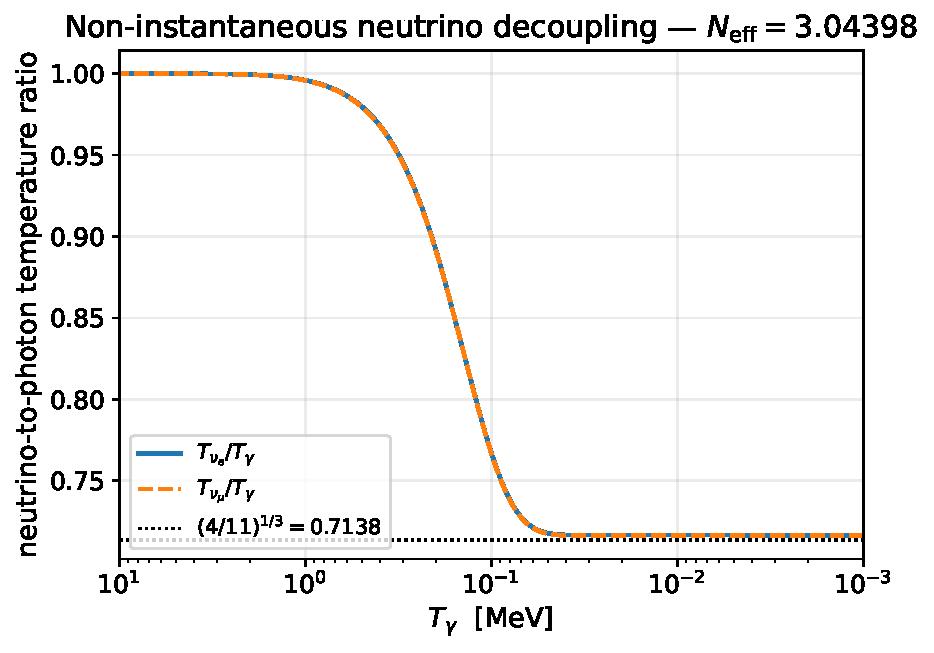
\includegraphics[width=0.70\textwidth]{plasma_neutrino_decoupling.pdf}
  \caption{Per-flavour neutrino-to-photon temperature ratios from the NEVO
    non-instantaneous decoupling history. The dotted line is the instantaneous
    limit $(4/11)^{1/3}$; the residual offset is what raises $\Neff$ above~3.}
  \label{fig:decoupling}
\end{figure}

\begin{figure}[ht]
  \centering
  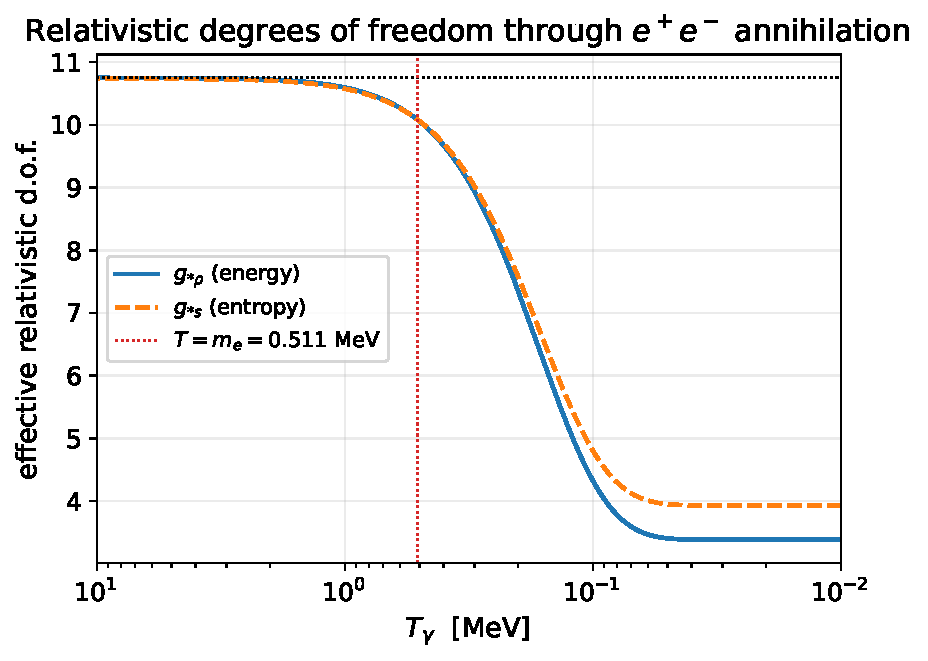
\includegraphics[width=0.70\textwidth]{plasma_gstar.pdf}
  \caption{Effective relativistic degrees of freedom in energy ($g_{*\rho}$) and
    entropy ($g_{*s}$), dropping from $10.75$ to $\simeq3.36/3.93$ as $e^+e^-$
    annihilate around $T\sim m_e$, heating the photons relative to the
    neutrinos.}
  \label{fig:gstar}
\end{figure}

\begin{figure}[ht]
  \centering
  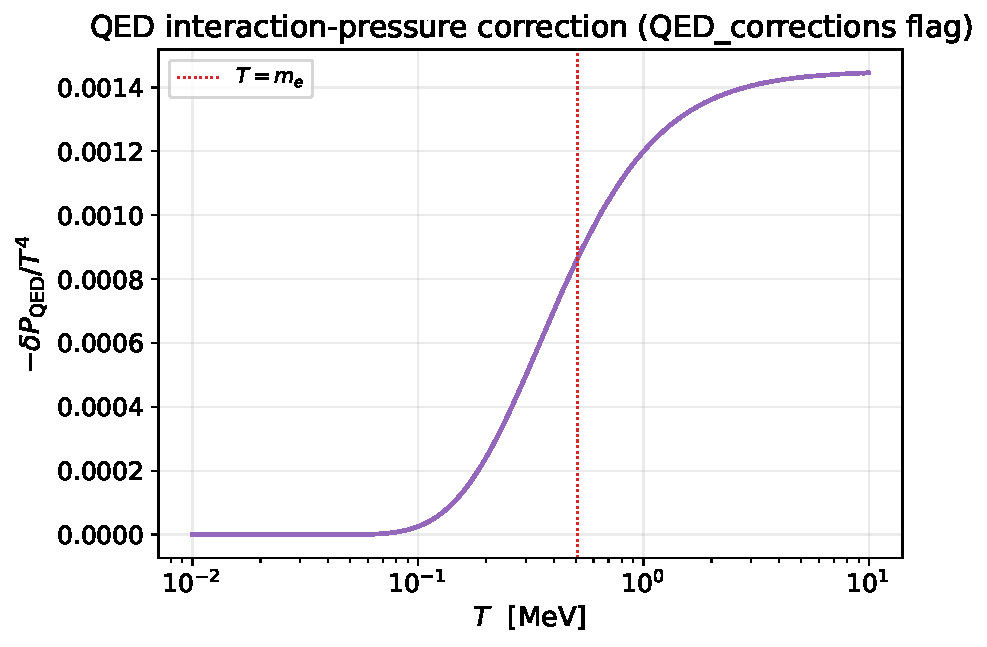
\includegraphics[width=0.62\textwidth]{plasma_qed_pressure.pdf}
  \caption{Leading QED interaction-pressure correction $-\delta P_{\rm QED}/T^4$,
    peaking near $T\sim m_e$; its size is set by $\afs/\pi$ (toggled by
    \code{QED\_corrections}).}
  \label{fig:qed}
\end{figure}

\subsection{Associated options}
\begin{center}\small
\begin{tabular}{>{\ttfamily}l l >{\raggedright\arraybackslash}p{8.4cm}}
\toprule
\normalfont Option & Default & Effect \\
\midrule
incomplete\_decoupling & True  & Use the NEVO non-instantaneous $\Tnu(\Tg)$ table (else instantaneous). \\
QED\_corrections       & True  & Include the QED plasma corrections (App.~\ref{app:qed}). \\
n\_electron\_table     & 2000  & Grid points for the $e^\pm$ thermodynamic tables. \\
recompute\_qed\_corrections & False & Recompute and overwrite \code{rates/plasma/QED\_*.txt}. \\
external\_background   & False & Read $a(\Tg)$ directly from the NEVO table instead of solving the ODE. \\
DeltaNeff              & 0     & Extra decoupled radiation added to $\rho_{\rm tot}$. \\
munuOverTnu            & 0     & Neutrino degeneracy $\xi_\nu=\mu_\nu/\Tnu$. \\
\bottomrule
\end{tabular}
\end{center}

% =====================================================================
\section{Weak interactions}\label{sec:weak}
% =====================================================================

\subsection{The six processes and their rates}
The neutron-to-proton ratio is controlled by six weak processes related by
crossing symmetry (\PR\ Eq.~67),
\begin{equation}
  n+\nu_e \leftrightarrow p+e^-, \quad
  n \leftrightarrow p+e^-+\bar\nu_e, \quad
  n+e^+ \leftrightarrow p+\bar\nu_e,
\label{eq:sixprocesses}
\end{equation}
grouped into a forward rate $\Gamma_{n\to p}$ (sum of the three) and a reverse
$\Gamma_{p\to n}$. Each rate is a phase-space integral over the weak matrix
element with the appropriate Fermi--Dirac occupations and Pauli-blocking factors
(\PR\ Eq.~70; App.~\ref{app:weak}, Eq.~\eqref{eq:weakgen}). The neutron-proton
density evolution is
\begin{equation}
  \dot n_n + 3Hn_n = -n_n\Gamma_{n\to p} + n_p\Gamma_{p\to n}.
\end{equation}

\subsection{Born approximation and calibration}
In the infinite-nucleon-mass (Born) limit the matrix element collapses to a
constant and the forward rate becomes the one-dimensional integral (\PR\
Eqs.~77--83)
\begin{equation}
  \overline\Gamma_{n\to p} = \Kw\!\int_0^\infty\! p^2\,\dd p\,
     \big[\chi_+(E)+\chi_+(-E)\big],
  \quad
  \chi_\pm(E)\equiv (E_\nu^\mp)^2\,g_\nu(E_\nu^\mp)\,g(-E),
\label{eq:born}
\end{equation}
with $E=\sqrt{p^2+m_e^2}$, $E_\nu^\mp=E\mp\Gap$, $\Gap=m_n-m_p$, $g$ and $g_\nu$
the electron and neutrino Fermi--Dirac distributions at $T$ and $\Tnu$, and the
normalisation
\begin{equation}
  \Kw = \frac{4\,G_W^2(1+3g_A^2)}{(2\pi)^3}, \qquad G_W = G_F\cos\theta_C .
\label{eq:K}
\end{equation}
Because $G_W$ and $g_A$ carry $\sim\!10^{-3}$ uncertainties, $\Kw$ is instead
fixed by the measured free-neutron lifetime through $\Kw=1/(\tau_n\lambda_0
m_e^5)$, where $\lambda_0$ is the dimensionless decay phase-space integral (\PR\
Eqs.~89--91); its value rises from $\bar\lambda_0\simeq1.636$ (Born) to
$\lambda_0^{\rm RC+FM}\simeq1.7547$ once corrections are included
(App.~\ref{app:weak}). When $\Tnu=T$ the rates obey the detailed-balance
relation $\overline\Gamma_{p\to n}=e^{-\Gap/T}\overline\Gamma_{n\to p}$, which
the code preserves order by order.

\subsection{Corrections beyond Born}
Reproducing $\YP$ to $10^{-3}$ requires several corrections, applied in sequence
(full formulas in App.~\ref{app:weak}):
\begin{enumerate}\itemsep2pt
  \item \emph{$T=0$ radiative corrections}: a Coulomb (Fermi) factor
    $\mathcal{F}_\pm(E)$ multiplying the integrand when electron and proton are
    on the same side, times the resummed radiative factor
    $R(E,k_{\max})=1+\frac{\afs}{2\pi}\mathcal{C}(E,k_{\max})$ built from
    Sirlin's universal function (\PR\ Eqs.~98--101; the Marciano--Sirlin
    resummation of \cite{Czarnecki2004}). Largest single effect,
    $\Delta\YP\simeq+0.2\%$.
  \item \emph{Bremsstrahlung}: real-photon emission, added to keep detailed
    balance consistent with the finite-$T$ terms (\PR\ \S III.E.2).
  \item \emph{Finite-temperature radiative corrections}: stimulated
    emission/absorption and the electron energy shift in the thermal bath
    (Brown \& Sawyer \cite{BrownSawyer}; \PR\ \S III.G), split into three pieces
    $\Gamma^{\gamma,T}+\Gamma^{\Delta E,T}+\Gamma^{ep+ee,T}$.
  \item \emph{Finite nucleon mass}: a Fokker--Planck expansion to first order in
    $T/m_N$ giving $\chi^{\rm FM}_\pm$ (\PR\ \S III.F; App.~\ref{app:weak}).
  \item \emph{Weak magnetism}: at order $T/m_N$ it is equivalent to a shift of
    the chiral couplings $\cLL\to\cLL+f_{\rm wm}g_A$, $\cRR\to\cRR-f_{\rm wm}g_A$
    with $f_{\rm wm}=(\mu_p-\mu_n)/2\simeq1.853$ (\PR\ \S III.F; Seckel
    \cite{Seckel1993}).
  \item \emph{Neutrino spectral distortions}: the equilibrium $g_\nu$ is replaced
    by the actual NEVO neutrino spectrum, which is slightly out of equilibrium.
\end{enumerate}
Figure~\ref{fig:weakrates} compares the calibrated rates with $H$, and
Fig.~\ref{fig:weakcorr} decomposes the total correction to $\Gamma_{n\to p}$: the
$T=0$ radiative/finite-mass/weak-magnetism block dominates ($\sim\!-4$ to
$-6\%$), while the finite-$T$ and spectral pieces are sub-percent.
Figure~\ref{fig:xn} shows the resulting neutron history.

\begin{figure}[ht]
  \centering
  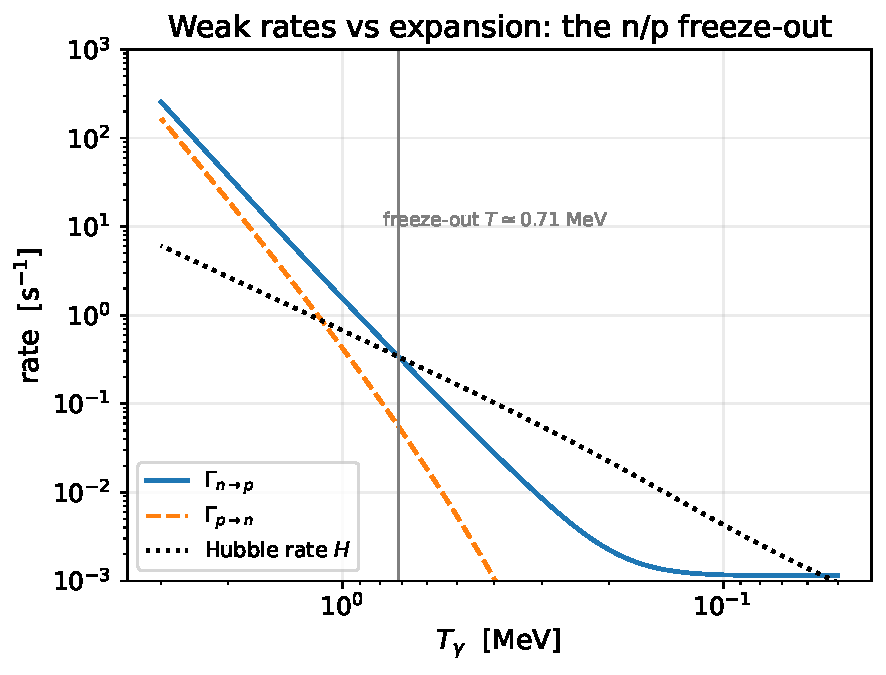
\includegraphics[width=0.70\textwidth]{weak_rates_vs_hubble.pdf}
  \caption{Calibrated weak rates and the Hubble rate $H$. Equilibrium holds where
    $\Gamma>H$; the high-$T$ crossing is the $n/p$ freeze-out. (Time flows left
    to right.)}
  \label{fig:weakrates}
\end{figure}

\begin{figure}[ht]
  \centering
  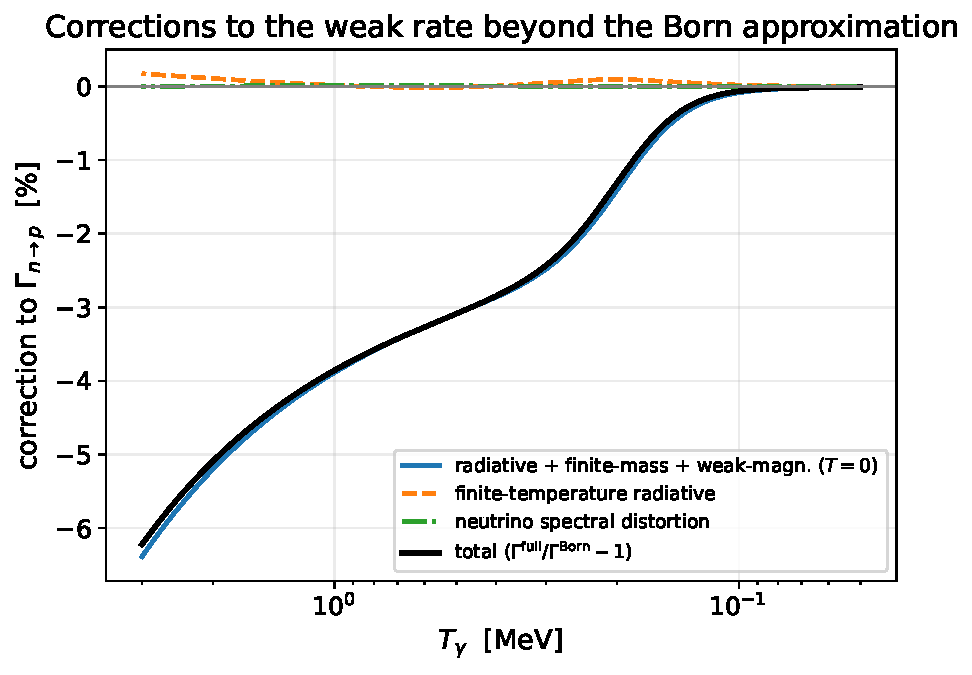
\includegraphics[width=0.76\textwidth]{weak_corrections_breakdown.pdf}
  \caption{Decomposition of the correction to $\Gamma_{n\to p}$ relative to the
    Born rate, obtained by toggling the corresponding flags. The $T=0$ block
    (radiative + finite-mass + weak-magnetism) dominates; finite-temperature and
    spectral-distortion contributions are at the per-mille level.}
  \label{fig:weakcorr}
\end{figure}

\begin{figure}[ht]
  \centering
  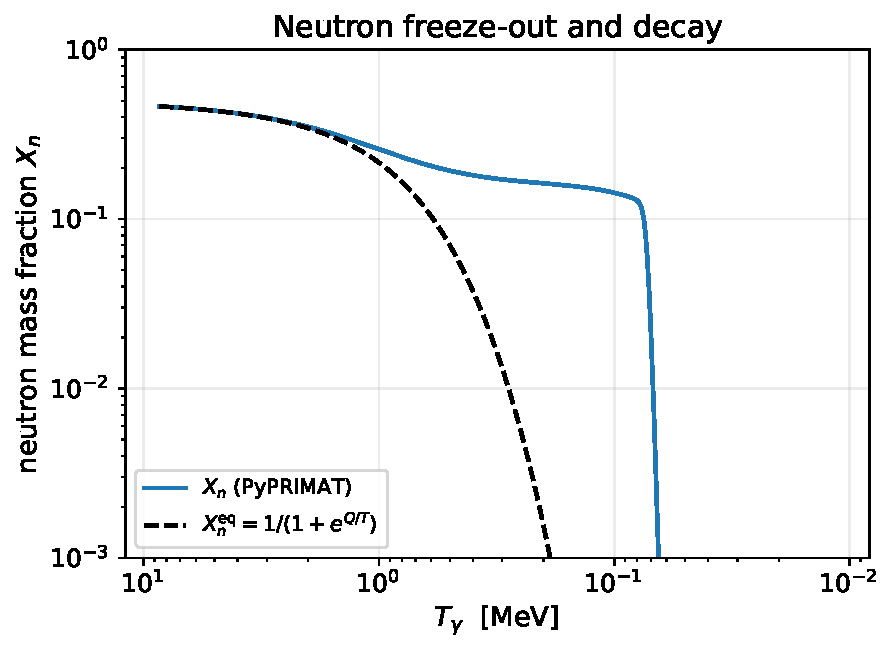
\includegraphics[width=0.66\textwidth]{weak_neutron_fraction.pdf}
  \caption{Neutron mass fraction $X_n$ from PyPRIMAT (solid) versus the
    weak-equilibrium prediction $X_n^{\rm eq}=1/(1+e^{Q/T})$ (dashed). $X_n$
    tracks equilibrium until freeze-out near $0.8$~MeV, then declines slowly
    until deuterium formation burns the neutrons into $^4$He.}
  \label{fig:xn}
\end{figure}

\subsection{In the code}
\code{weak\_rates.py} evaluates Eq.~\eqref{eq:born} and all corrections on the
background grid. Results are cached in \code{rates/weak/} behind a configuration
\emph{fingerprint}, so a rerun with the same physics reloads them while a changed
configuration recomputes. The normalisation $1/(\tau_n\lambda_0 m_e^5)$ is stored
as \code{\_NormWeakRates} and the temperature interpolants are
\code{\_nTOp\_frwrd}/\code{\_nTOp\_bkwrd} (argument in kelvin).

\subsection{Associated options}
\begin{center}\small
\begin{tabular}{>{\ttfamily}l l >{\raggedright\arraybackslash}p{8.4cm}}
\toprule
\normalfont Option & Default & Effect \\
\midrule
tau\_n                  & 878.4 & Neutron lifetime [s] used to calibrate $\Kw$. \\
tau\_n\_flag            & True  & Normalise via $\tau_n$ (else from $G_F$, $V_{ud}$, $g_A$). \\
nTOp\_Born\_approximation & False & Use only the Born rate (debugging/comparison). \\
include\_nTOp\_thermal  & True  & Apply the finite-temperature radiative correction. \\
spectral\_distortions   & True  & Use the actual NEVO neutrino spectrum in the rates. \\
sampling\_nTOp          & 200   & Points in the $n\leftrightarrow p$ rate grid. \\
weak\_rate\_cache       & True  & Reuse the fingerprinted \code{rates/weak/} cache when valid. \\
\bottomrule
\end{tabular}
\end{center}

% =====================================================================
\section{Nuclear reactions}\label{sec:nuclear}
% =====================================================================

\subsection{Thermal averaging of reaction rates}
In the plasma the nuclei have a Maxwell--Boltzmann distribution of relative
velocities (\PR\ Eq.~118), and the thermonuclear rate of a two-body reaction is
the thermal average of the cross-section (\PR\ Eq.~119),
\begin{equation}
  \NA\sigmav = \NA\!\int_0^\infty\!\sigma(v)\,\phi_{\rm MB}(v)\,v\,\dd v,
  \qquad
  \phi_{\rm MB}(v)\,v\,\dd v = \sqrt{\tfrac{8}{\pi m}}\,
     \frac{E\,e^{-E/k_BT}}{(k_BT)^{3/2}}\,\dd E,
\label{eq:thermalavg}
\end{equation}
in $\mathrm{cm^3\,s^{-1}\,mol^{-1}}$, with $m$ the reduced mass. For
charged-particle reactions $\sigma$ is dominated by Coulomb-barrier tunnelling,
so it is written with the astrophysical $S$-factor
$\sigma(E)=S(E)\,e^{-2\pi\eta}/E$, where $\eta=Z_1Z_2 e^2/(\hbar v)$ is the
Sommerfeld parameter (\PR\ Eqs.~120--122); $S(E)$ removes most of the energy
dependence except for resonances. PyPRIMAT does not perform this average at run
time: it reads the precomputed $\NA\sigmav(T_9)$ tables (from the NACRE-II and
related evaluations \cite{NACRE2,Coc2012}) and resamples them onto a common $T_9$
grid (log--log cubic interpolation). Five radiative-capture rates
($n(p,\gamma)d$, $d(p,\gamma)^3$He, $t(p,\gamma)^4$He, $t(\alpha,\gamma)^7$Li,
$^3$He$(\alpha,\gamma)^7$Be) additionally receive a $T_9$-dependent QED
correction (\code{nuclear\_qed\_corrections}; Pitrou \& Pospelov
\cite{PitrouPospelov2020}), applied as a multiplicative rescaling of the median
rate at load time so that the corrected value becomes the new central rate.

\subsection{The reaction network}
With $Y_i\equiv n_i/n_b$ (so $\sum_i A_iY_i=1$), baryon conservation removes the
dilution term and the abundances obey the Wagoner form (\PR\ Eqs.~130--132)
\begin{equation}
  \dot Y_{i} = \sum_{\text{reactions}} N_i\!\left[
      \Gamma_{\!j\to i}\,
      \frac{\textstyle\prod_j Y_j^{N_j}}{\textstyle\prod_j N_j!}
    - \Gamma_{\!i\to j}\,
      \frac{\textstyle\prod_i Y_i^{N_i}}{\textstyle\prod_i N_i!}\right],
\label{eq:network}
\end{equation}
where $N_i$ is the stoichiometric coefficient of species $i$ and the abundance
rate is related to the number-density rate by
$\Gamma_{i_1\dots\to\dots}=n_b^{(\sum N_i)-1}\,\gamma$ with
$\gamma=\sigmav$. For the common two-body case $i+j\leftrightarrow k+l$ this is
\begin{equation}
  \dot Y_i \supset Y_kY_l\,\Gamma_{kl\to ij} - Y_iY_j\,\Gamma_{ij\to kl},
  \qquad \Gamma_{ij\to kl}=n_b\,\sigmav_{ij\to kl}.
\end{equation}

\paragraph{Symmetry factors.}
The factorials $N_i!$ in Eq.~\eqref{eq:network} are the combinatorial symmetry
factors that appear whenever a reaction has \emph{identical} reactants or
products. For example $d+d\to {}^3\mathrm{He}+n$ has two identical deuterons in
the entrance channel ($N_d=2$): the number of distinct reacting pairs in a gas
of $n_d$ deuterons is $\tfrac12 n_d(n_d-1)\simeq\tfrac12 n_d^2$, so the flux
carries a factor $1/2!=1/2$, and the stoichiometric prefactor $N_d=2$ means each
reaction removes two deuterons. The same $1/N!$ appears for identical products
(e.g. $^7\mathrm{Li}+p\to\alpha+\alpha$). Omitting these factors would
double-count indistinguishable pairs.

\subsection{Reverse rates from detailed balance}
Only forward rates are tabulated; reverse rates are fixed by requiring that at
nuclear statistical equilibrium (NSE) forward and reverse fluxes cancel. Using
the equilibrium number densities (App.~\ref{app:nse}) the ratio depends only on
the nuclide masses, spins and the reaction $Q$-value, and takes the
three-parameter form (\PR\ Eqs.~135--137)
\begin{equation}
  \frac{\gamma_{kl\to ij}}{\gamma_{ij\to kl}}
    = \alpha\left(\frac{T}{10^9\,\mathrm K}\right)^{\!\beta}
      \exp\!\left(\frac{\gamma\times10^9\,\mathrm K}{T}\right),
\label{eq:detbal}
\end{equation}
with $(\alpha,\beta,\gamma)$ computed once per reaction from nuclide data
(\texttt{compute\_detailed\_\allowbreak balance\_coefficients}). The derivation, including the
symmetry factors and the binding-energy exponent, is given in
App.~\ref{app:nse}. Figure~\ref{fig:rates} shows several forward rates together
with their reverse (photo-dissociation) rates: the reverse rate rises steeply
with $T_9$ and crosses the forward rate around $T_9\sim1$--$2$, i.e. where each
capture is balanced by its inverse -- this is the bottleneck that holds the
nuclei at their NSE values until the universe cools enough.

\subsection{The three-era ODE integration}\label{sec:eras}
The full network is far too stiff to integrate in one shot, so the solve is
split at the fixed boundaries
$T_{\rm start}(10\,\mathrm{MeV})>T_{\rm weak}(\sim\!0.8\,\mathrm{MeV})>
T_{\rm nucl}(\sim\!0.08\,\mathrm{MeV})>T_{\rm end}(\sim\!10^{-3}\,\mathrm{MeV})$,
mapped to times through $t(T)$:
\begin{itemize}\itemsep2pt
  \item \textbf{HT era} ($T_{\rm start}\!\to\!T_{\rm weak}$): only $n,p$, governed
    by the linear system
    $\dot Y_n=b\,Y_p-f\,Y_n$, $\dot Y_p=f\,Y_n-b\,Y_p$ with
    $f=\Gamma_{n\to p}$, $b=\Gamma_{p\to n}$, started from weak equilibrium
    $Y_n=b/(b+f)$ and integrated with the non-stiff LSODA solver.
  \item \textbf{MT era} ($T_{\rm weak}\!\to\!T_{\rm nucl}$): the fixed
    18-reaction subset (even for medium/large -- the full net is too stiff before
    the deuterium bottleneck opens), seeded with the HT $\{Y_n,Y_p\}$ and the NSE
    values $Y_i^{\rm NSE}$ (App.~\ref{app:nse}) for all other species, integrated
    with the implicit BDF solver and the analytic Jacobian.
  \item \textbf{LT era} ($T_{\rm nucl}\!\to\!T_{\rm end}$): the full chosen
    network (12 / 62 / $\sim$433 reactions), seeded from the MT result, BDF +
    Jacobian.
\end{itemize}
The normalised $n\!\leftrightarrow\!p$ rates feed all three eras as
$f,b=\text{NormWR}\times\{$\code{\_nTOp\_frwrd},\code{\_nTOp\_bkwrd}$\}$ with
$\text{NormWR}=1/(\tau_n F_n)$ in the \code{tau\_n\_flag} mode ($F_n$ the decay
phase-space factor). The reverse nuclear rates of Eq.~\eqref{eq:detbal} are
clamped at low $T_9$ so that the exothermic factor $e^{\gamma/T_9}$ cannot
overflow (the ``exothermic blow-up'' guard in \code{nuclear.py}).

\paragraph{Solvers and the Jacobian.}
Two of \code{scipy.integrate.solve\_ivp}'s integrators are used. \textbf{LSODA}
(the Livermore solver with automatic stiffness detection) switches on the fly
between a non-stiff Adams--Moulton predictor--corrector and a stiff backward
formula; it is used for the smooth, mildly-stiff \emph{background} ODEs
[$a(T)$ of Eq.~\eqref{eq:aofT} and $t(a)$] and for the two-species HT system.
The MT and LT \emph{nuclear} networks are very stiff -- a fast reaction and its
detailed-balance reverse differ by many orders of magnitude, so the Jacobian has
widely separated eigenvalues -- and are integrated with the implicit
\textbf{BDF} method (backward differentiation formulas), which is
unconditionally stable for stiff systems where an explicit method would need
prohibitively small steps. A BDF step solves a nonlinear system by Newton
iteration and therefore needs the Jacobian
$J_{ij}=\partial\dot Y_i/\partial Y_j$ of the right-hand
side~\eqref{eq:network}. Rather than let the solver estimate $J$ by finite
differences (costly and noisy for $\sim$60 species), PyPRIMAT supplies it
analytically: \code{compile\_network} differentiates the polynomial mass-action
terms symbolically and emits a fast \code{njit} kernel
(\code{nucl.JacobianMT}/\code{JacobianLT}), passed to \code{solve\_ivp} via its
\code{jac} argument, which both accelerates and stabilises the integration.

\subsection{Final observables}\label{sec:obs}
At $T_{\rm end}$ the code forms the nine entries of the result dictionary:
\begin{equation}
  \YP^{\rm BBN}=4Y_{^4{\rm He}},\quad
  \DoH=\frac{Y_{\rm D}}{Y_p},\quad
  \frac{^3{\rm He}}{\rm H}=\frac{Y_{^3{\rm H}}+Y_{^3{\rm He}}}{Y_p},\quad
  \frac{^7{\rm Li}}{\rm H}=\frac{Y_{^7{\rm Li}}+Y_{^7{\rm Be}}}{Y_p},
\end{equation}
where $^3$H$+^3$He and $^7$Be$+^7$Li include the post-BBN $\beta$-decays
$^3$H$\to{}^3$He and $^7$Be$\to{}^7$Li. $\Neff$ is read off the
neutrino-to-photon energy ratio at $T_{\rm end}$ via Eq.~\eqref{eq:neff};
$\YP^{\rm CMB}$ is the helium mass fraction \emph{by mass} (using the
$^4$He/$^1$H mass ratio) as relevant for CMB analyses; and \code{Omeganurel} /
\code{OneOverOmeganunr} are the relativistic relic-neutrino $\Omega_\nu h^2$ and
the inverse non-relativistic $\Omega_\nu h^2$ per summed eV, built from the
$T_\nu/\Tg$ ratio at $T_{\rm end}$ scaled to today through $T_0^{\rm CMB}$.

\subsection{Networks, eras, and rate variation}
The reaction list is named in
\code{rates/nuclear/networks/\{small,medium,large\}.txt}; \code{load\_network}
parses it and \code{compile\_network} turns the stoichiometry of
Eq.~\eqref{eq:network} into fast right-hand-side and Jacobian kernels (the three
eras of Sec.~\ref{sec:eras} share these kernels).
Each reaction \code{<name>} carries a variation knob \code{p\_<name>} sampling
its rate at $\text{median}\times e^{p\,\sigma}$ for Monte-Carlo error
propagation; the additive \code{NP\_delta\_<name>} (with
\code{rescale\_nuclear\_rates=True}) multiplies it by $1+\delta$:
\begin{lstlisting}[style=py]
PyPR({"network": "medium", "p_dpTOHe3g": 1.0}).solve()   # d(p,gamma)He3 at +1 sigma
\end{lstlisting}
Figure~\ref{fig:evol} shows the abundance history and Fig.~\ref{fig:schramm} the
final abundances versus the baryon density with the observational constraints.

\begin{figure}[ht]
  \centering
  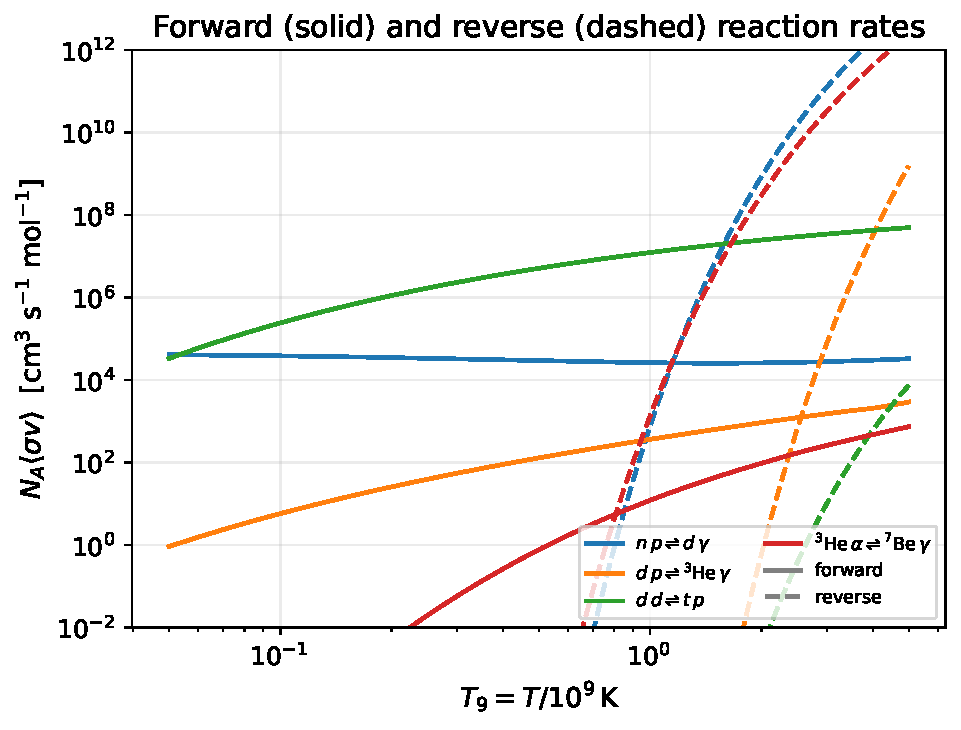
\includegraphics[width=0.72\textwidth]{nuclear_reaction_rates.pdf}
  \caption{Forward (solid) and reverse (dashed, by detailed balance) rates
    $\NA\sigmav(T_9)$ for four key reactions. The forward rates depend only
    weakly on $T_9$; the reverse photo-dissociation rates rise steeply and cross
    the forward rates near $T_9\sim1$--$2$.}
  \label{fig:rates}
\end{figure}

\begin{figure}[ht]
  \centering
  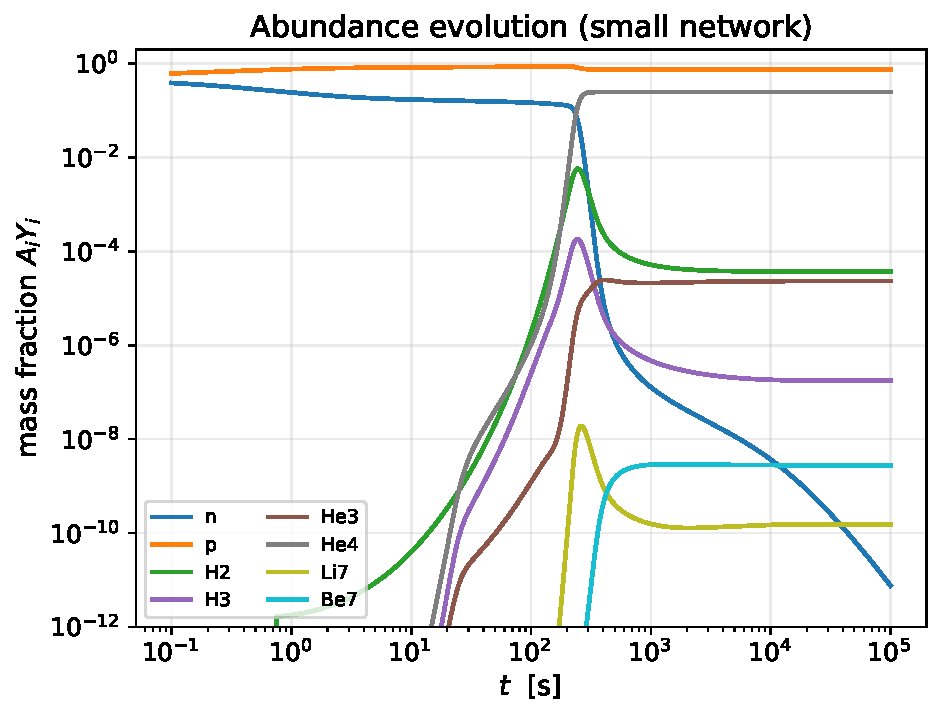
\includegraphics[width=0.72\textwidth]{nuclear_abundance_evolution.pdf}
  \caption{Mass fractions $A_iY_i(t)$ for the small network. Deuterium builds up
    and is rapidly burned into $^4$He once $T\sim0.07$~MeV (the deuterium
    bottleneck), leaving the trace primordial D, $^3$He, $^7$Li and $^7$Be.}
  \label{fig:evol}
\end{figure}

\begin{figure}[ht]
  \centering
  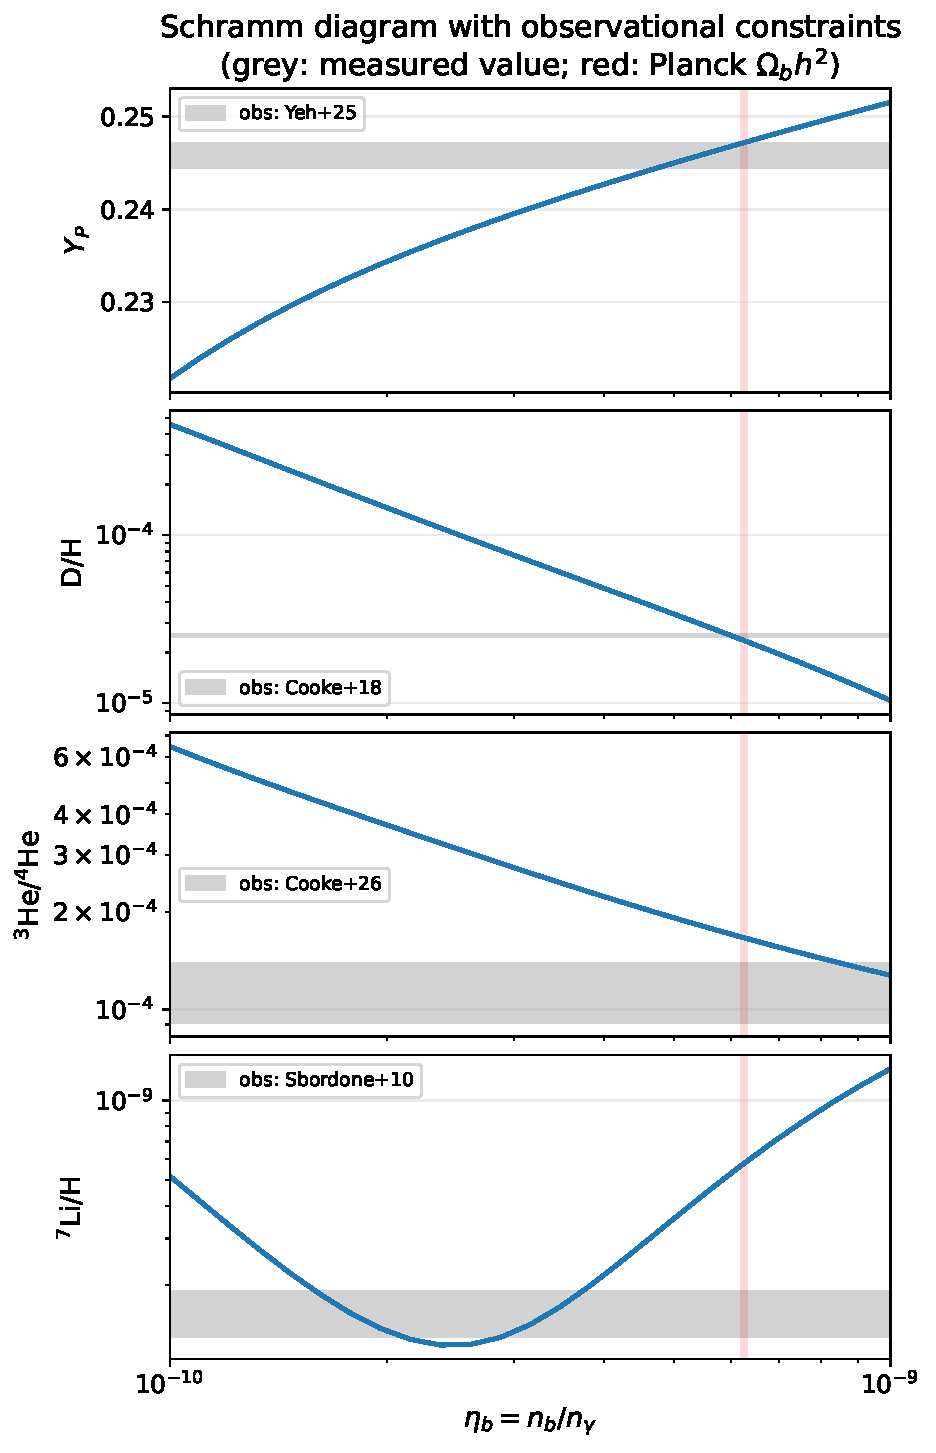
\includegraphics[width=0.52\textwidth]{nuclear_schramm.pdf}
  \caption{Schramm diagram with observational constraints (grey bands; values
    from \code{notebooks/StandardPlots.ipynb}). The red band is the Planck baryon
    density. $\YP$ and D/H agree with Planck, $^3$He/$^4$He lies somewhat high,
    and $^7$Li/H is over-predicted -- the ``lithium problem''.}
  \label{fig:schramm}
\end{figure}

\subsection{Rate uncertainties}
Each evaluated rate comes with a $1\sigma$ uncertainty (a log-normal width
$\sigma$ per reaction). These propagate to the abundances; the dominant ones for
$\YP$ are the neutron lifetime and the $n(p,\gamma)d$, $d(d,n)^3$He,
$d(d,p)t$ reactions, with the rule-of-thumb (\PR\ Eq.~145)
\begin{equation}
  \Delta\YP \approx 1.5\times10^{-3}\,
     \frac{\Delta\sigmav}{\sigmav}, \qquad
  \Delta\YP \approx 0.18\,\frac{\Delta\tau_n}{\tau_n},
\end{equation}
while D/H is most sensitive to $d(p,\gamma)^3$He, $d(d,n)^3$He and $d(d,p)t$. In
PyPRIMAT the full budget is obtained by Monte-Carlo, drawing each \code{p\_<rxn>}
from $\mathcal N(0,1)$; the helper \code{mc\_uncertainty} parallelises this.
Section~\ref{sec:sensitivity} quantifies the individual responses.

\subsection{Associated options}
\begin{center}\small
\begin{tabular}{>{\ttfamily}l l >{\raggedright\arraybackslash}p{8.4cm}}
\toprule
\normalfont Option & Default & Effect \\
\midrule
network                 & "small" & Reaction set: \code{small} (12), \code{medium} (62), \code{large} ($\sim$433). \\
amax                    & None    & With \code{large}, drop nuclides of mass number $> A$. \\
nuclear\_qed\_corrections & True  & QED corrections to radiative-capture rates \cite{PitrouPospelov2020}. \\
numerical\_precision    & 1e-7    & Relative tolerance of the ODE solver. \\
rate\_grid\_npts        & 500     & Points in the master $T_9$ grid for rate resampling. \\
p\_<reaction>           & 0       & Log-normal variation of an individual rate (MCMC). \\
output\_time\_evolution & False   & Write the full time series to \code{results/output\_tables.tsv}. \\
\bottomrule
\end{tabular}
\end{center}

% =====================================================================
\section{Sensitivity of the abundances}\label{sec:sensitivity}
% =====================================================================
A compact way to understand which inputs matter is the logarithmic sensitivity
\begin{equation}
  S(O,p) \equiv \frac{\partial\ln O}{\partial\ln p}
  \approx \frac{\ln O(p(1+\delta)) - \ln O(p(1-\delta))}{2\ln(1+\delta)},
\end{equation}
the percentage change of observable $O$ per percent change of parameter $p$,
evaluated by a symmetric $\delta=1\%$ finite difference. Figure~\ref{fig:sens}
shows the matrix for the four light-element observables against the twelve key
reaction rates and the physical parameters $\tau_n$, $G_N$, $\Omega_bh^2$ and
$\Delta\Neff$. Reading it off: $\YP$ is almost insensitive to the nuclear rates
but responds strongly to $\Delta\Neff$ (faster expansion $\to$ earlier
freeze-out $\to$ more neutrons) and to $\tau_n$; D/H is driven by $\Omega_bh^2$,
$G_N$ and the deuterium-burning rates; $^7$Li/H is anti-correlated with
$\Omega_bh^2$ along the upper Schramm branch and sensitive to the
$^3$He$(\alpha,\gamma)^7$Be and $^7$Be$(n,p)^7$Li rates. The figure reproduces
\code{notebooks/Sensitivity.ipynb}.

\begin{figure}[ht]
  \centering
  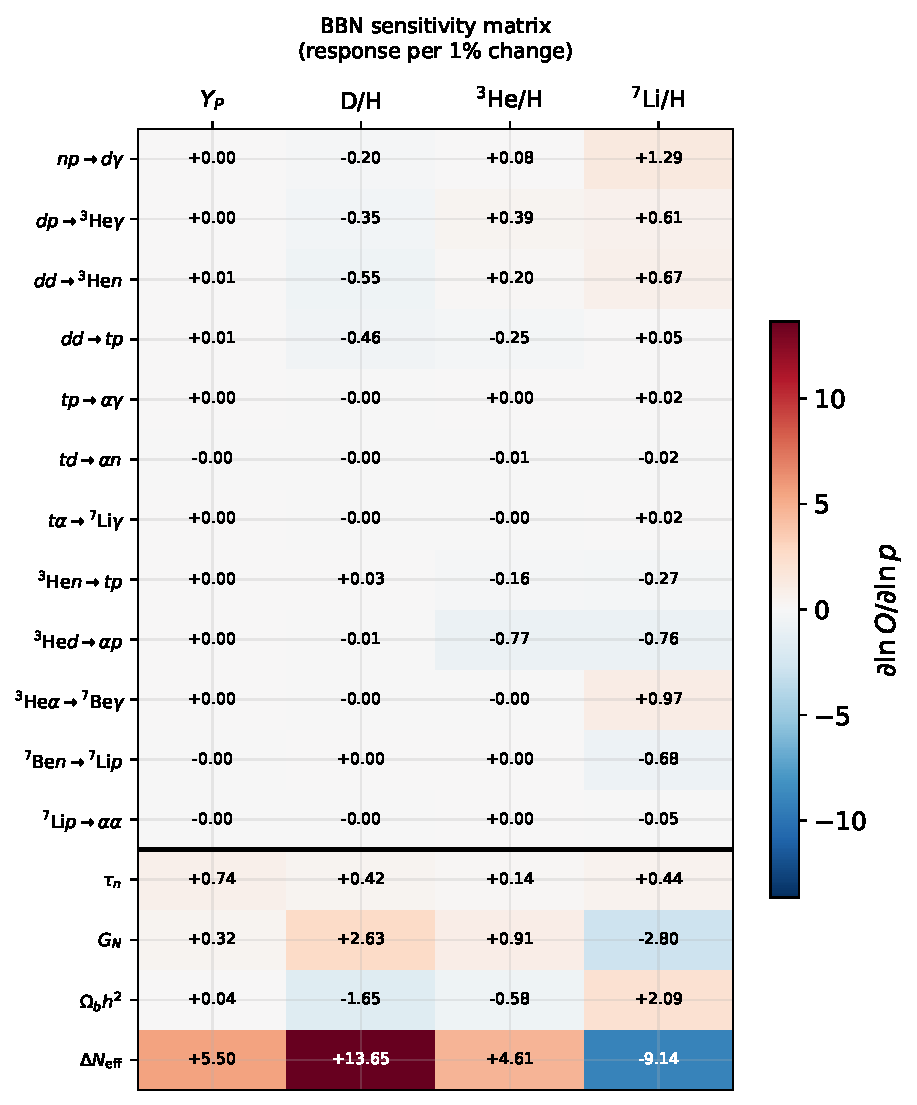
\includegraphics[width=0.66\textwidth]{sensitivity_heatmap.pdf}
  \caption{Logarithmic sensitivity $\partial\ln O/\partial\ln p$ of the four
    observables (columns) to the nuclear rates (top block) and physical
    parameters (bottom block), per $1\%$ change. Red is positive, blue negative.}
  \label{fig:sens}
\end{figure}

% =====================================================================
\appendix
\section{Thermodynamic integrals}\label{app:thermo}
% =====================================================================
The Fermi--Dirac ($+$) and Bose--Einstein ($-$) integrals used in
Eq.~\eqref{eq:thermo} are (\PR\ App.~A)
\begin{equation}
  I^{(n,m)}_\pm(x) \equiv \int_0^\infty
     \frac{p^{\,n}\,\mathcal{E}^{\,m-n}}{e^{\mathcal{E}}\pm1}\,\dd p,
  \qquad \mathcal{E}\equiv\sqrt{p^2+x^2},\ \ x=m/T,
\end{equation}
so that $\rho=\frac{gT^4}{2\pi^2}I^{(2,1)}_\pm$, $P=\frac{gT^4}{6\pi^2}
I^{(0,3)}_\pm$ and $n=\frac{gT^3}{2\pi^2}I^{(2,0)}_\pm$. Useful limits are
$I^{(2,1)}_+(0)=\tfrac{7\pi^4}{120}$, $I^{(0,1)}_+(0)=\tfrac{\pi^2}{12}$ and
$I^{(0,1)}_-=\tfrac{\pi^2}{6}$. The electron chemical potential is non-zero only
through the tiny charge-neutrality constraint $n_{e^-}-n_{e^+}=n_p$ and is
neglected ($\xi_e\ll1$) in the weak rates; it is kept only where it sets the
absolute $e^\pm$ number density.

% =====================================================================
\section{QED plasma corrections}\label{app:qed}
% =====================================================================
The thermal $e^\pm$/photon interactions shift the masses by (\PR\ Eqs.~40, 42;
\cite{Mangano2001,LopezTurner1998})
\begin{equation}
\begin{aligned}
  \frac{\delta m_e^2(p,T)}{T^2} &= \frac{4\afs}{\pi}\big[I^{(0,1)}_- + I^{(0,1)}_+(x)\big]
     - \frac{2\bar m_e^2\afs}{\pi\bar p}\!\int_0^\infty\!\dd\bar q\,
       \frac{\bar q}{\mathcal{E}_{\bar q}}
       \ln\!\Big|\frac{\bar p+\bar q}{\bar p-\bar q}\Big|\,
       \frac{1}{e^{\mathcal{E}_{\bar q}}+1},\\
  \frac{\delta m_\gamma^2}{T^2} &= \frac{8\afs}{\pi}I^{(0,1)}_+(x),
\end{aligned}
\end{equation}
with $\bar p=p/T$, $x=\bar m_e=m_e/T$, $\mathcal{E}_{\bar q}=\sqrt{\bar q^2+x^2}$.
The induced pressure shift is a sum of three terms in increasing order of the
electromagnetic coupling $e$ (with $\afs=e^2/4\pi$). PyPRIMAT
(\code{qed\_pressure.py}) tabulates and \emph{sums the first two}, stored as the
two columns of \code{rates/plasma/QED\_*.txt}:
\begin{align}
  \frac{\delta P_a}{T^4} &= \frac{\afs}{\pi}\!\left[
     -\frac{2}{3}I^{(0,1)}_+(x) - \frac{2}{\pi^2}\big(I^{(0,1)}_+(x)\big)^2\right]
     && [O(e^2),\ \text{dominant, negative}],\\
  \frac{\delta P_{e^3}}{T^4} &= \frac{4}{3}\sqrt{2\pi}\,\afs^{3/2}
     \left[\frac{I^{(0,1)}_+(x)+I^{(2,-1)}_+(x)}{\pi^2}\right]^{3/2}
     && [O(e^3),\ \text{ring/plasmon}],\\
  \frac{\delta P_b}{T^4} &= \frac{\afs}{\pi^3}\,\bar m_e^2\!
     \iint\!\frac{\bar p^2\,\dd\bar p}{\mathcal{E}_{\bar p}}
     \frac{\bar q^2\,\dd\bar q}{\mathcal{E}_{\bar q}}
     \ln\!\Big|\frac{\bar p+\bar q}{\bar p-\bar q}\Big|
     \frac{1}{(e^{\mathcal{E}_{\bar p}}+1)(e^{\mathcal{E}_{\bar q}}+1)}
     && [O(e^4),\ \text{optional}],
\end{align}
with $I^{(2,-1)}_+(x)=\int_0^\infty\!\sqrt{p^2+x^2}/(e^{\mathcal{E}}+1)\,\dd p$
(\code{I2m1}). $\delta P_a$ is the one-loop Frenkel--Galitskii--Migdal term, the
$O(\afs^{3/2})$ ring term $\delta P_{e^3}$ is the Blaizot--Zinn-Justin plasmon
resummation (PRIMAT-Main.m), and the two-loop exchange $\delta P_b$ -- equal to
the subdominant integral $\overline{\delta P}_{\rm s}$ of \PR\ Eq.~49 -- is
\emph{off by default} (it would need a separate flag/file). The energy shift
follows from $\rho=-P+T\,\dd P/\dd T$,
\begin{equation}
  \overline{\delta\rho} = 3\,\overline{\delta P}
     + \frac{\partial\,\overline{\delta P}}{\partial\ln T},
  \qquad
  \delta g_\rho \equiv \frac{30}{\pi^2}\overline{\delta\rho},\quad
  \delta g_P \equiv \frac{90}{\pi^2}\overline{\delta P},
\end{equation}
with the high-$T$ limit $\delta g_\rho\simeq\delta g_P\simeq-25\afs/(4\pi)$. These
enter the code in four places (\PR\ Eqs.~50--53): (i) the plasma entropy
$\mathcal{S}^{\rm QED}=\mathcal{S}+(\delta g_P+3\delta g_\rho)/8$ used to obtain
$a(T)$; (ii) the neutrino-temperature normalisation
$(z_0^{\rm QED})^3=\tfrac{11}{4}(1-\tfrac{4}{11}\tfrac{25\afs}{8\pi})$, giving
$z_0^{\rm QED}\simeq1.39979$; (iii) the plasma energy density
$\mathcal{E}^{\rm QED}=\mathcal{E}+\delta g_\rho/2$ in
Eq.~\eqref{eq:friedmann}; and (iv) through the electron mass shift -- which is
exactly the Brown--Sawyer relation $2E\,\Delta E=\delta m_e^2$ and is therefore
counted as a finite-temperature weak-rate correction (App.~\ref{app:weak}).

% =====================================================================
\section{Weak rates beyond the Born approximation}\label{app:weak}
% =====================================================================

\subsection*{Matrix element}
With the mostly-minus signature, each rate with nucleon $a$ in the initial and
$b$ in the final state is (\PR\ Eq.~A40)
\begin{equation}
  n_a\Gamma_{a\to b} = \int\frac{\dd^3\mathbf p_a\,\dd^3\mathbf p_e\,\dd^3\mathbf p_\nu}
     {2^4(2\pi)^8}\,
     \delta(E_a-E_b+s_eE_e+s_\nu E_\nu)\,
     \frac{|M|^2_{a\to b}}{E_nE_pE_eE_\nu}\,
     f_a f_\nu(s_\nu E_\nu) f_e(s_e E_e),
\label{eq:weakgen}
\end{equation}
where $s_{e,\nu}=+1$ ($-1$) for an initial (final) lepton, and a final-state
lepton enters as a Pauli-blocking factor via $f(-E)=1-f(E)$. The interaction is
$\mathcal H_I=\tfrac{G_F}{\sqrt2}J^\mu_{e\nu}J_{pn,\mu}$ with a purely
left-chiral leptonic current and the hadronic current (\PR\ Eqs.~A41--A44)
\begin{equation}
  J^\mu_{pn} = \cos\theta_C\,\bar p\!\left(\gamma^\mu(1-g_A\gamma^5)
    + \ii\frac{f_{\rm wm}}{m_N}2\Sigma^{\mu\nu}q_\nu\right)\! n,
  \qquad f_{\rm wm}=\frac{\mu_p-\mu_n}{2}\simeq1.853 .
\end{equation}
Ignoring weak magnetism, the squared matrix element is
$\tfrac{|M|^2}{2^7G_F^2}=\cLL\mathcal M_{LL}+\cRR\mathcal M_{RR}+\cLR\mathcal M_{LR}$
with
\begin{equation}
  \cLL=\tfrac{(1+g_A)^2}{4},\quad
  \cRR=\tfrac{(1-g_A)^2}{4},\quad
  \cLR=\tfrac{g_A^2-1}{4},
\end{equation}
and $\mathcal M_{LL}=(p_n\!\cdot\!p_\nu)(p_p\!\cdot\!p_e)$,
$\mathcal M_{RR}=(p_n\!\cdot\!p_e)(p_p\!\cdot\!p_\nu)$,
$\mathcal M_{LR}=m_pm_n(p_\nu\!\cdot\!p_e)$ (\PR\ Eq.~A46). All six processes of
Eq.~\eqref{eq:sixprocesses} share this matrix element (crossing + time reversal).

\subsection*{Born rate and calibration}
In the infinite-mass limit the three $\mathcal M/(E_nE_pE_eE_\nu)\to1$ (after an
angular average), giving Eqs.~\eqref{eq:born}--\eqref{eq:K}. The decay
phase-space factor is (\PR\ Eq.~88)
\begin{equation}
  \bar\lambda_0 = m_e^{-5}\!\int_0^{\sqrt{\Gap^2-m_e^2}}\! p^2 E_\nu^2\,\dd p
   = \sqrt{\bar\Gap^2-1}\,\frac{-8-9\bar\Gap^2+2\bar\Gap^4}{60}
     + \frac{\bar\Gap}{4}\mathrm{arccosh}\,\bar\Gap \simeq 1.63609,
\end{equation}
with $\bar\Gap=\Gap/m_e$; including radiative and finite-mass corrections raises
it to $\lambda_0^{\rm RC+FM}\simeq1.75474$.

\subsection*{$T=0$ radiative corrections}
The corrected forward rate is (\PR\ Eq.~99)
\begin{equation}
  \Gamma^{\mathrm{RC}0}_{n\to p}=\Kw\!\int_0^\infty\! p^2\,\dd p\,
    \big[\mathcal F_+(E)R(E,E_\nu)\chi_+(E)
        +\mathcal F_+(-E)R(E,\Gap+E)\chi_+(-E)\big],
\end{equation}
where the Fermi (Coulomb) factor $\mathcal F_\pm(x)=F(|x|)$ if $\pm x>0$ and $1$
otherwise switches on only when the electron and proton are on the same side.
The radiative factor is $R(E,k_{\max})=1+\frac{\afs}{2\pi}\mathcal C(E,k_{\max})$
with Sirlin's function (\PR\ Eqs.~A78--A80; \cite{Sirlin1967})
\begin{align}
  \mathcal C(E,k_{\max}) &= 4\ln\frac{m_Z}{m_p}+\ln\frac{m_p}{m_A}+2C+A_g
     + g(E,k_{\max}),\\
  g(E,k_{\max}) &= 3\ln\frac{m_p}{m_e}-\frac34
     + \frac{4}{\beta}L\!\Big(\frac{2\beta}{1+\beta}\Big)
     + 4[R(\beta)-1]\!\Big[\frac{k_{\max}}{3E}-\frac32+\ln\frac{2k_{\max}}{m_e}\Big]
     \nonumber\\
     &\quad + R(\beta)\Big[2(1+\beta^2)+\frac{k_{\max}^2}{6E^2}-4\beta R(\beta)\Big],
\end{align}
with $\beta=p/E$, $R(\beta)=\tfrac{1}{2\beta}\ln\tfrac{1+\beta}{1-\beta}$,
$L[x]=\int_0^x\tfrac{\ln(1-t)}{t}\dd t$ the Spence function, and the constants
$C\simeq0.891$, $A_g\simeq-0.34$, $m_A\simeq1.2$~GeV. By default the code uses
the Marciano--Sirlin resummed form (\PR\ Eq.~A81; \cite{Czarnecki2004})
\begin{equation}
  R(E,k_{\max}) = \Big[1+\tfrac{\afs}{2\pi}\big(g(E,k_{\max})-3\ln\tfrac{m_p}{2\Gap}\big)\Big]
    \Big(L+\tfrac{\afs}{\pi}C+\tfrac{\afs}{2\pi}\delta\Big)
    \Big[S+\tfrac{\afs(m_p)}{2\pi}\big(\ln\tfrac{m_p}{m_A}+A_g\big)+\text{NLL}\Big],
\end{equation}
with $L\simeq1.02094$, $S\simeq1.02248$, $\afs(m_p)\simeq1/134$. The reverse rate
uses $\chi_+\to\chi_-$, $\mathcal F_+\to\mathcal F_-$, preserving detailed balance.

\subsection*{Bremsstrahlung and finite-temperature corrections}
To keep detailed balance once the thermal bath is included, the
neutron-beta-decay bremsstrahlung is re-added consistently (\PR\ Eq.~100). The
finite-temperature radiative correction has three parts (\PR\ Eqs.~104--106;
\cite{BrownSawyer}),
$\Gamma^{T}=\Gamma^{\gamma,T}+\Gamma^{\Delta E,T}+\Gamma^{ep+ee,T}$. The
photon-exchange part is
\begin{equation}
  \Gamma^{\gamma,T}_{n\to p}=\frac{\afs\Kw}{2\pi}\!\int_0^\infty\!\frac{\dd k}{k}
    \!\int_{m_e}^\infty\!\dd E\,
    \Big\{A(E,k)\big[g(-E)\tilde\chi^A_+(E,k)+g(E)\tilde\chi^A_+(-E,k)\big]
    - kB(E,k)\big[\dots\big]\Big\},
\end{equation}
with $\tilde\chi^A_\pm(E,k)=\tilde\chi_\pm(E-k)+\tilde\chi_\pm(E+k)-2\tilde\chi_\pm(E)$
and $\tilde\chi^B_\pm(E,k)=\pm[\tilde\chi_\pm(E-k)-\tilde\chi_\pm(E+k)]$; the
electron-energy-shift part is
\begin{equation}
  \Gamma^{\Delta E,T}_{n\to p}=-\frac{2\afs\Kw}{\pi}\!\int\!\dd p\,
    [\chi_+(E)+\chi_+(-E)]
    \Big[\frac{\pi^2T^2}{6}+\!\int_{m_e}^\infty\!\dd E'\,p'g(E')
    \Big(1-\frac{m_e^2}{E'^2-E^2}\Big)\Big].
\end{equation}
These integrals are evaluated with the \code{vegas} Monte-Carlo library (or
\code{scipy.dblquad}) and cached.

\subsection*{Finite nucleon mass and weak magnetism}
The Born rate drops terms $E_\nu/m_N$, $E_e/m_N$, $\Gap/m_N$, all of order
$\epsilon\equiv T/m_N\sim10^{-3}$ near freeze-out. PyPRIMAT keeps them to first
order in $\epsilon$ (neglecting $O(\epsilon^2)\sim10^{-6}$) through a
Fokker--Planck expansion of Eq.~\eqref{eq:weakgen} in the energy transferred to
the leptons, which adds (\PR\ Eq.~94)
\begin{equation}
  \delta\Gamma^{\rm FM}_{n\to p}
   = \Kw\!\int_0^\infty\! p^2\,\dd p\,
     [\chi^{\rm FM}_+(E,g_A)+\chi^{\rm FM}_+(-E,g_A)],
\end{equation}
with $\Gamma_{p\to n}$ obtained by $\chi^{\rm FM}_+(E,g_A)\to\chi^{\rm
FM}_-(E,-g_A)$. Because finite-mass and radiative corrections are both
percent-level and do not add linearly, the multiplicative radiative factor
$\mathcal F_\pm(E)\,R(E,k_{\max})$ is also applied to the finite-mass integrand
($\delta\Gamma^{\rm RC+FM}$, \PR\ Eq.~95). The kernel $\chi^{\rm FM}_\pm(E,g_A)$
(\PR\ Eq.~A66) is built from the derivatives
$g^{(n,p)}_\nu(E_\nu)\equiv\partial_{E_\nu}^p[E_\nu^n g_\nu(E_\nu)]$ and the
reduced couplings $\tilde c_{..}=\tfrac{4}{1+3g_A^2}c_{..}$; its $T=0$ limit
(which enters the calibration $\lambda_0$) is
\begin{equation}
  \chi^{\rm FM}_+|_{T=0} = \tilde\cLL\frac{p^2E_\nu^2}{m_NE}
    + \tilde\cRR\frac{E_\nu^3}{m_N}
    - (\tilde\cLL+\tilde\cRR+\tilde\cLR)\frac{2E_\nu^3+E_\nu p^2}{m_N}
    + \tilde\cLR\frac{p^2E_\nu^2}{m_NE}.
\end{equation}
Weak magnetism, at this order, is equivalent to the shift
\begin{equation}
  \cLL\to\frac{(1+g_A)^2}{4}+f_{\rm wm}g_A, \qquad
  \cRR\to\frac{(1-g_A)^2}{4}-f_{\rm wm}g_A, \qquad
  \cLR \text{ unchanged},
\end{equation}
so it is implemented simply by modifying the couplings entering
$\chi^{\rm FM}_\pm$ (\PR\ \S III.F; \cite{Seckel1993}). Combined with radiative
corrections it shifts $\lambda_0$ by $\delta\lambda_0^{\rm FM}\simeq-3.63\times
10^{-3}$.

\subsection*{Spectral distortions}
Finally, the equilibrium $g_\nu$ in $\chi_\pm$ is replaced by the actual neutrino
occupation $f_\nu=g_\nu+\delta f_\nu$, which deviates from a Fermi--Dirac because
of incomplete decoupling (\code{spectral\_distortions=True}). PyPRIMAT supports
two forms of $\delta f_\nu$ (\code{neutrino\_history.py}):
\begin{itemize}\itemsep2pt
  \item \emph{NEVO-table} (default, \code{analytic\_distortions=False}): the
    distortion is read from the full NEVO spectrum file as a function of comoving
    momentum $y=E_\nu/T_\nu$ and $\Tg$.
  \item \emph{Analytic} $\mu$/$y$ (\code{analytic\_distortions=True}; requires
    instantaneous decoupling), two continuous knobs \code{delta\_xi\_nu} and
    \code{y\_SZ}:
    \begin{align}
      \delta f^\mu_\nu(y) &= \frac{1}{e^{\,y-(\xi+\delta\xi)}+1}-\frac{1}{e^{\,y-\xi}+1}
        && (\mu\text{-type, shift of }\xi=\mu_\nu/T_\nu),\\
      \delta f^y_\nu(y) &= f_{\rm FD}(1-f_{\rm FD})\,[\,4-y(1-2f_{\rm FD})\,]
        && (y\text{-type / SZ}),
    \end{align}
    where $f_{\rm FD}=1/(e^y+1)$; the $y$-type shape is
    $y^{-2}\,\dd_y(y^4\,\dd_y f_{\rm FD})$, the Sunyaev--Zel'dovich form. The same
    distortion adds an energy density $\rho_\nu^{\rm SD}$ to the Friedmann
    equation~\eqref{eq:friedmann}.
\end{itemize}

% =====================================================================
\section{Detailed balance and nuclear statistical equilibrium}\label{app:nse}
% =====================================================================
At thermal equilibrium a non-relativistic species has number density (\PR\
Eq.~A33)
\begin{equation}
  n_i = g_i\Big(\frac{m_iT}{2\pi}\Big)^{3/2}e^{\xi_i-x_i},
  \qquad g_i=2s_i+1,\ \ \xi_i=\mu_i/T,\ \ x_i=m_i/T .
\end{equation}
At NSE a nuclide is in chemical equilibrium with its nucleons,
$\mu_i=Z_i\mu_p+(A_i-Z_i)\mu_n$, which gives (\PR\ Eq.~A35)
\begin{equation}
  n_i^{\rm NSE} = \frac{g_i m_i^{3/2}}{2^{A_i}}
    \Big(\frac{n_p}{m_p^{3/2}}\Big)^{Z_i}
    \Big(\frac{n_n}{m_n^{3/2}}\Big)^{A_i-Z_i}
    \Big(\frac{2\pi}{T}\Big)^{3(A_i-1)/2} e^{B_i/T},
  \qquad B_i = Z_im_p+(A_i-Z_i)m_n-m_i,
\end{equation}
with $B_i$ the binding energy. Requiring forward and reverse fluxes to cancel at
NSE, the general detailed-balance relation is (\PR\ Eq.~133)
\begin{equation}
  \frac{\gamma_{i_1\dots i_p\to j_1\dots j_q}}{\gamma_{j_1\dots j_q\to i_1\dots i_p}}
   = \frac{N_{i_1}!\cdots N_{i_p}!}{N_{j_1}!\cdots N_{j_q}!}
     \left[\frac{n_{j_1}^{N_{j_1}}\cdots}{n_{i_1}^{N_{i_1}}\cdots}\right]^{\rm NSE},
\end{equation}
where the factorials are exactly the symmetry factors of
Eq.~\eqref{eq:network}. Substituting $n_i^{\rm NSE}$ and using that nuclear
reactions conserve $Z$ and $A$ (so the $n_p,n_n$ powers cancel) leaves a function
of masses, spins and $T$ only (\PR\ Eq.~134),
\begin{equation}
  \frac{\gamma_{j\to i}}{\gamma_{i\to j}}
   = \frac{\prod_i \tfrac{1}{N_i!}\big[g_i(m_iT/2\pi)^{3/2}\big]^{N_i}}
          {\prod_j \tfrac{1}{N_j!}\big[g_j(m_jT/2\pi)^{3/2}\big]^{N_j}}\,
     \exp\!\Big(\frac{\sum_j m_j-\sum_i m_i}{T}\Big),
\end{equation}
which collapses to the three-constant form of Eq.~\eqref{eq:detbal}: $\alpha$
gathers the spin/mass/$2\pi$ prefactors, $\beta=\tfrac{3}{2}(\sum N_i-\sum N_j)$
the power of $T$, and $\gamma\propto$ the reaction $Q$-value $\sum_j m_j-\sum_i
m_i$. The masses and spins are taken from the AME/NUBASE tables
\cite{AME2016}. PyPRIMAT computes $(\alpha,\beta,\gamma)$ once per reaction in
\code{compute\_detailed\_balance\_coefficients} and stores them in
\code{rates/nuclear/data/detailed\_balance.csv}.

% =====================================================================
\section{Nuclear reaction list and sources}\label{app:reactions}
% =====================================================================
PyPRIMAT's networks are plain lists of reaction names under
\code{rates/nuclear/networks/} (the \code{small}, \code{medium} and
\code{large} files); each name maps to a rate table under
\code{rates/nuclear/tables/} whose header line records the
reaction and a short source code \code{ref=...}.
Tables~\ref{tab:rxn-small}--\ref{tab:rxn-large} reproduce every reaction,
expanded as $a+b\leftrightarrow c+d$ (each tabulated forward rate is supplemented
by its detailed-balance reverse, App.~\ref{app:nse}), with that source code.
Throughout, $a\equiv{}^4$He ($\alpha$), $d\equiv{}^2$H, $t\equiv{}^3$H,
$g\equiv\gamma$, $n,p$ the nucleons, and $e^\mp$ the leptons of $\beta$-decays
(one-way, shown with $\to$). A $^\dagger$ marks rates that are analytic fits
hard-coded in PRIMAT-Main.m; ``(borrowed)'' marks a rate set equal to another
reaction's.

The source codes follow the convention ``\textsc{Aaa}\,YY'' = first-author
prefix + year (e.g. \texttt{And06} = Ando et al.\ 2006). The principal ones are:
\textbf{And06} Ando et al.\ (2006, $n(p,\gamma)d$ EFT);
\textbf{Moscoso2021} Moscoso et al.\ (2021);
\textbf{Gom17} G\'omez I\~nesta, Iliadis \& Coc (2017);
\textbf{Ser04} Serpico et al.\ (2004);
\textbf{Ili16} Iliadis et al.\ (2016);
\textbf{deSouza19a/b}, \textbf{deSouza2020} de Souza, Iliadis \& Coc (2019, 2020);
\textbf{DAACV04} Descouvemont, Adahchour, Angulo, Coc \& Vangioni (2004);
\textbf{NACRE II} Xu et al.\ (2013) \cite{NACRE2};
\textbf{NACRE} Angulo et al.\ (1999);
\textbf{ILCCF10} Iliadis, Longland, Champagne, Coc \& Fitzgerald (2010);
\textbf{CGXSV12} Coc, Goriely, Xu, Saimpert \& Vangioni (2012) \cite{Coc2012};
\textbf{TALYS2} the TALYS statistical-model code (Koning et al.);
\textbf{CF88} Caughlan \& Fowler (1988);
\textbf{MF89} Malaney \& Fowler (1989);
\textbf{Rau94} Rauscher et al.\ (1994);
\textbf{Wag69} Wagoner (1969);
\textbf{Aud03} Audi, Wapstra \& Thibault (2003, $\beta$-decay/mass data);
\textbf{Trezzi2017} Trezzi et al.\ (LUNA, 2017);
\textbf{Bar16} Barbagallo et al.\ (n\_TOF, 2016);
\textbf{Rij19} Rijal et al.\ (2019).
The remaining short author--year codes -- almost all carrying the $^\dagger$
analytic-fit marker (\texttt{Bal95}, \texttt{Bar97C}, \texttt{Efr96},
\texttt{FK90}, \texttt{Has09c}, \texttt{Iga95}, \texttt{Kaw91}, \texttt{Koe91},
\texttt{Men12}, \texttt{Nag06}, \texttt{Tang03}, \texttt{Wan91},
\texttt{Wie87/89}, \texttt{TUNL\&Cam08}, \texttt{MF89\&Hei98},
\texttt{Des99Bea01}) -- decode by the same first-author/year rule, but their
full bibliographic entries are not reproduced here; they are catalogued in the
compilations of Coc et al.\ \cite{Coc2012} and the NACRE/NACRE-II evaluations
\cite{NACRE2} and are not all individually retrievable from the shipped tables.

\begin{center}\scriptsize
\setlength{\tabcolsep}{3pt}
\begin{longtable}{@{}r l l @{\hspace{0.4em}} r l l@{}}
\caption{Small network (12 reactions). $^\dagger$ = analytic fit hard-coded in PRIMAT-Main.m.}\label{tab:rxn-small}\\
\toprule
\# & Reaction & Source & \# & Reaction & Source\\\midrule
\endfirsthead
\multicolumn{6}{r}{\footnotesize\itshape table~\ref{tab:rxn-small} continued}\\\toprule
\# & Reaction & Source & \# & Reaction & Source\\\midrule
\endhead
\bottomrule
\endfoot
1 & $n + p \leftrightarrow d + \gamma$ & And06 & 7 & $t + \alpha \leftrightarrow {}^{7}\mathrm{Li} + \gamma$ & DAACV04\\
2 & $d + p \leftrightarrow {}^{3}\mathrm{He} + \gamma$ & Moscoso2021 & 8 & ${}^{3}\mathrm{He} + n \leftrightarrow t + p$ & DAACV04\\
3 & $d + d \leftrightarrow {}^{3}\mathrm{He} + n$ & Gom17 & 9 & ${}^{3}\mathrm{He} + d \leftrightarrow \alpha + p$ & deSouza19b\\
4 & $d + d \leftrightarrow t + p$ & Gom17 & 10 & ${}^{3}\mathrm{He} + \alpha \leftrightarrow {}^{7}\mathrm{Be} + \gamma$ & Ili16\\
5 & $t + p \leftrightarrow \alpha + \gamma$ & Ser04 & 11 & ${}^{7}\mathrm{Be} + n \leftrightarrow {}^{7}\mathrm{Li} + p$ & deSouza2020\\
6 & $t + d \leftrightarrow \alpha + n$ & deSouza19a & 12 & ${}^{7}\mathrm{Li} + p \leftrightarrow \alpha + \alpha$ & DAACV04\\
\end{longtable}
\end{center}

\begin{center}\scriptsize
\setlength{\tabcolsep}{3pt}
\begin{longtable}{@{}r l l @{\hspace{0.4em}} r l l@{}}
\caption{\code{large} network additions at \code{amax=8} beyond the small network (55 reactions): this is the exact reaction set of the former \code{medium} network, reproduced by \code{\{\"network\": \"large\", \"amax\": 8\}}.}\label{tab:rxn-medium}\\
\toprule
\# & Reaction & Source & \# & Reaction & Source\\\midrule
\endfirsthead
\multicolumn{6}{r}{\footnotesize\itshape table~\ref{tab:rxn-medium} continued}\\\toprule
\# & Reaction & Source & \# & Reaction & Source\\\midrule
\endhead
\bottomrule
\endfoot
1 & ${}^{8}\mathrm{B} \to \alpha + \alpha + e^+$ & Aud03$^\dagger$ & 29 & ${}^{6}\mathrm{Li} + n \leftrightarrow t + \alpha$ & CF88$^\dagger$\\
2 & ${}^{8}\mathrm{B} + d \leftrightarrow {}^{7}\mathrm{Be} + {}^{3}\mathrm{He}$ & TALYS2 & 30 & ${}^{6}\mathrm{Li} + p \leftrightarrow {}^{7}\mathrm{Be} + \gamma$ & NACRE II\\
3 & ${}^{8}\mathrm{B} + n \leftrightarrow {}^{7}\mathrm{Be} + d$ & TALYS2 & 31 & ${}^{6}\mathrm{Li} + p \leftrightarrow {}^{3}\mathrm{He} + \alpha$ & NACRE II\\
4 & ${}^{8}\mathrm{B} + n \leftrightarrow {}^{6}\mathrm{Li} + {}^{3}\mathrm{He}$ & TALYS2 & 32 & ${}^{6}\mathrm{Li} + t \leftrightarrow {}^{7}\mathrm{Li} + d$ & TALYS2\\
5 & ${}^{8}\mathrm{B} + n \leftrightarrow \alpha + \alpha + p$ & TALYS2 & 33 & ${}^{6}\mathrm{Li} + t \leftrightarrow {}^{8}\mathrm{Li} + p$ & TALYS2\\
6 & ${}^{8}\mathrm{B} + t \leftrightarrow {}^{7}\mathrm{Be} + \alpha$ & TALYS2 & 34 & ${}^{6}\mathrm{Li} + t \leftrightarrow \alpha + \alpha + n$ & TALYS2\\
7 & ${}^{8}\mathrm{B} + t \leftrightarrow \alpha + \alpha + {}^{3}\mathrm{He}$ & TALYS2 & 35 & ${}^{7}\mathrm{Li} + {}^{3}\mathrm{He} \leftrightarrow {}^{6}\mathrm{Li} + \alpha$ & TALYS2\\
8 & ${}^{7}\mathrm{Be} + {}^{3}\mathrm{He} \leftrightarrow \alpha + \alpha + p + p$ & CF88\&MF89$^\dagger$ & 36 & ${}^{7}\mathrm{Li} + {}^{3}\mathrm{He} \leftrightarrow \alpha + \alpha + d$ & TALYS2\\
9 & ${}^{7}\mathrm{Be} + {}^{3}\mathrm{He} \leftrightarrow p + p + \alpha + \alpha$ & TALYS2 & 37 & ${}^{7}\mathrm{Li} + {}^{3}\mathrm{He} \leftrightarrow \alpha + \alpha + n + p$ & CF88\&MF89$^\dagger$\\
10 & ${}^{7}\mathrm{Be} \to {}^{7}\mathrm{Li} + e^+$ & Aud03$^\dagger$ & 38 & ${}^{7}\mathrm{Li} + d \leftrightarrow {}^{8}\mathrm{Li} + p$ & MF89$^\dagger$\\
11 & ${}^{7}\mathrm{Be} + d \leftrightarrow \alpha + \alpha + p$ & Rij19 & 39 & ${}^{7}\mathrm{Li} + d \leftrightarrow \alpha + \alpha + n$ & CGXSV12\\
12 & ${}^{7}\mathrm{Be} + n \leftrightarrow \alpha + \alpha$ & Bar16 & 40 & ${}^{7}\mathrm{Li} + n \leftrightarrow {}^{8}\mathrm{Li} + \gamma$ & MF89\&Hei98$^\dagger$\\
13 & ${}^{7}\mathrm{Be} + p \leftrightarrow {}^{8}\mathrm{B} + \gamma$ & NACRE II & 41 & ${}^{7}\mathrm{Li} + p \leftrightarrow \alpha + \alpha + \gamma$ & NACRE II\\
14 & ${}^{7}\mathrm{Be} + t \leftrightarrow {}^{6}\mathrm{Li} + \alpha$ & TALYS2 & 42 & ${}^{7}\mathrm{Li} + t \leftrightarrow \alpha + \alpha + n + n$ & CF88\&MF89$^\dagger$\\
15 & ${}^{7}\mathrm{Be} + t \leftrightarrow {}^{7}\mathrm{Li} + {}^{3}\mathrm{He}$ & TALYS2 & 43 & ${}^{8}\mathrm{Li} + {}^{3}\mathrm{He} \leftrightarrow {}^{7}\mathrm{Li} + \alpha$ & TALYS2\\
16 & ${}^{7}\mathrm{Be} + t \leftrightarrow \alpha + \alpha + d$ & TALYS2 & 44 & ${}^{8}\mathrm{Li} + {}^{3}\mathrm{He} \leftrightarrow \alpha + \alpha + t$ & TALYS2\\
17 & ${}^{7}\mathrm{Be} + t \leftrightarrow \alpha + \alpha + n + p$ & CF88\&MF89$^\dagger$ & 45 & ${}^{8}\mathrm{Li} \to \alpha + \alpha + e^-$ & Aud03$^\dagger$\\
18 & ${}^{3}\mathrm{He} + {}^{3}\mathrm{He} \leftrightarrow \alpha + p + p$ & NACRE II & 46 & ${}^{8}\mathrm{Li} + d \leftrightarrow {}^{7}\mathrm{Li} + t$ & Has09c$^\dagger$\\
19 & ${}^{3}\mathrm{He} + n \leftrightarrow \alpha + \gamma$ & Wag69$^\dagger$ & 47 & ${}^{8}\mathrm{Li} + p \leftrightarrow \alpha + \alpha + n$ & Men12$^\dagger$\\
20 & ${}^{3}\mathrm{He} + t \leftrightarrow {}^{6}\mathrm{Li} + \gamma$ & FK90$^\dagger$ & 48 & $\alpha + n + n \leftrightarrow {}^{6}\mathrm{He} + \gamma$ & Efr96$^\dagger$\\
21 & ${}^{3}\mathrm{He} + t \leftrightarrow \alpha + d$ & CF88$^\dagger$ & 49 & $\alpha + n + p \leftrightarrow {}^{6}\mathrm{Li} + \gamma$ & CF88$^\dagger$\\
22 & ${}^{3}\mathrm{He} + t \leftrightarrow \alpha + n + p$ & CF88$^\dagger$ & 50 & $d + \alpha \leftrightarrow {}^{6}\mathrm{Li} + \gamma$ & Trezzi2017\\
23 & ${}^{6}\mathrm{He} \to {}^{6}\mathrm{Li} + e^-$ & Aud03$^\dagger$ & 51 & $d + d \leftrightarrow \alpha + \gamma$ & NACRE II\\
24 & ${}^{6}\mathrm{Li} + {}^{3}\mathrm{He} \leftrightarrow {}^{7}\mathrm{Be} + d$ & TALYS2 & 52 & $d + n \leftrightarrow t + \gamma$ & Nag06$^\dagger$\\
25 & ${}^{6}\mathrm{Li} + {}^{3}\mathrm{He} \leftrightarrow \alpha + \alpha + p$ & TALYS2 & 53 & $p + p + n \leftrightarrow d + p$ & CF88$^\dagger$\\
26 & ${}^{6}\mathrm{Li} + d \leftrightarrow {}^{7}\mathrm{Be} + n$ & MF89$^\dagger$ & 54 & $t \to {}^{3}\mathrm{He} + e^-$ & Aud03$^\dagger$\\
27 & ${}^{6}\mathrm{Li} + d \leftrightarrow {}^{7}\mathrm{Li} + p$ & MF89$^\dagger$ & 55 & $t + t \leftrightarrow \alpha + n + n$ & Nag06$^\dagger$\\
28 & ${}^{6}\mathrm{Li} + n \leftrightarrow {}^{7}\mathrm{Li} + \gamma$ & MF89$^\dagger$ & & &\\
\end{longtable}
\end{center}

\begin{center}\scriptsize
\setlength{\tabcolsep}{3pt}
\begin{longtable}{@{}r l l @{\hspace{0.4em}} r l l@{}}
\caption{Full \code{large} network additions beyond \code{amax=8} (361 reactions).}\label{tab:rxn-large}\\
\toprule
\# & Reaction & Source & \# & Reaction & Source\\\midrule
\endfirsthead
\multicolumn{6}{r}{\footnotesize\itshape table~\ref{tab:rxn-large} continued}\\\toprule
\# & Reaction & Source & \# & Reaction & Source\\\midrule
\endhead
\bottomrule
\endfoot
1 & ${}^{10}\mathrm{B} + {}^{3}\mathrm{He} \leftrightarrow {}^{11}\mathrm{C} + d$ & TALYS2 & 182 & ${}^{13}\mathrm{C} + {}^{3}\mathrm{He} \leftrightarrow {}^{15}\mathrm{N} + p$ & TALYS2\\
2 & ${}^{10}\mathrm{B} + {}^{3}\mathrm{He} \leftrightarrow {}^{12}\mathrm{C} + p$ & TALYS2 & 183 & ${}^{13}\mathrm{C} + {}^{3}\mathrm{He} \leftrightarrow {}^{15}\mathrm{O} + n$ & TALYS2\\
3 & ${}^{10}\mathrm{B} + {}^{3}\mathrm{He} \leftrightarrow {}^{12}\mathrm{N} + n$ & TALYS2 & 184 & ${}^{13}\mathrm{C} + {}^{3}\mathrm{He} \leftrightarrow {}^{16}\mathrm{O} + \gamma$ & TALYS2\\
4 & ${}^{10}\mathrm{B} + {}^{3}\mathrm{He} \leftrightarrow {}^{13}\mathrm{N} + \gamma$ & TALYS2 & 185 & ${}^{13}\mathrm{C} + \alpha \leftrightarrow {}^{16}\mathrm{O} + n$ & NACRE II\\
5 & ${}^{10}\mathrm{B} + \alpha \leftrightarrow {}^{12}\mathrm{C} + d$ & TALYS2 & 186 & ${}^{13}\mathrm{C} + \alpha \leftrightarrow {}^{17}\mathrm{O} + \gamma$ & TALYS2\\
6 & ${}^{10}\mathrm{B} + \alpha \leftrightarrow {}^{13}\mathrm{C} + p$ & TALYS2 & 187 & ${}^{13}\mathrm{C} + d \leftrightarrow {}^{11}\mathrm{B} + \alpha$ & TALYS2\\
7 & ${}^{10}\mathrm{B} + \alpha \leftrightarrow {}^{13}\mathrm{N} + n$ & CF88$^\dagger$ & 188 & ${}^{13}\mathrm{C} + d \leftrightarrow {}^{14}\mathrm{C} + p$ & TALYS2\\
8 & ${}^{10}\mathrm{B} + \alpha \leftrightarrow {}^{14}\mathrm{N} + \gamma$ & TALYS2 & 189 & ${}^{13}\mathrm{C} + d \leftrightarrow {}^{14}\mathrm{N} + n$ & TALYS2\\
9 & ${}^{10}\mathrm{B} + d \leftrightarrow {}^{11}\mathrm{B} + p$ & TALYS2 & 190 & ${}^{13}\mathrm{C} + d \leftrightarrow {}^{15}\mathrm{N} + \gamma$ & TALYS2\\
10 & ${}^{10}\mathrm{B} + d \leftrightarrow {}^{11}\mathrm{C} + n$ & TALYS2 & 191 & ${}^{13}\mathrm{C} + n \leftrightarrow {}^{14}\mathrm{C} + \gamma$ & TALYS2\\
11 & ${}^{10}\mathrm{B} + d \leftrightarrow {}^{12}\mathrm{C} + \gamma$ & TALYS2 & 192 & ${}^{13}\mathrm{C} + p \leftrightarrow {}^{14}\mathrm{N} + \gamma$ & NACRE II\\
12 & ${}^{10}\mathrm{B} + d \leftrightarrow \alpha + \alpha + \alpha$ & TALYS2 & 193 & ${}^{13}\mathrm{C} + t \leftrightarrow {}^{12}\mathrm{B} + \alpha$ & TALYS2\\
13 & ${}^{10}\mathrm{B} + n \leftrightarrow {}^{11}\mathrm{B} + \gamma$ & TALYS2 & 194 & ${}^{13}\mathrm{C} + t \leftrightarrow {}^{15}\mathrm{C} + p$ & TALYS2\\
14 & ${}^{10}\mathrm{B} + n \leftrightarrow {}^{10}\mathrm{Be} + p$ & TALYS2 & 195 & ${}^{13}\mathrm{C} + t \leftrightarrow {}^{15}\mathrm{N} + n$ & TALYS2\\
15 & ${}^{10}\mathrm{B} + n \leftrightarrow \alpha + \alpha + t$ & TALYS2 & 196 & ${}^{13}\mathrm{C} + t \leftrightarrow {}^{16}\mathrm{N} + \gamma$ & TALYS2\\
16 & ${}^{10}\mathrm{B} + p \leftrightarrow {}^{7}\mathrm{Be} + \alpha$ & NACRE II & 197 & ${}^{14}\mathrm{C} + {}^{3}\mathrm{He} \leftrightarrow {}^{13}\mathrm{C} + \alpha$ & TALYS2\\
17 & ${}^{10}\mathrm{B} + p \leftrightarrow {}^{11}\mathrm{C} + \gamma$ & NACRE II & 198 & ${}^{14}\mathrm{C} + {}^{3}\mathrm{He} \leftrightarrow {}^{16}\mathrm{N} + p$ & TALYS2\\
18 & ${}^{10}\mathrm{B} + p \leftrightarrow \alpha + \alpha + {}^{3}\mathrm{He}$ & TALYS2 & 199 & ${}^{14}\mathrm{C} + {}^{3}\mathrm{He} \leftrightarrow {}^{16}\mathrm{O} + n$ & TALYS2\\
19 & ${}^{10}\mathrm{B} + t \leftrightarrow {}^{11}\mathrm{B} + d$ & TALYS2 & 200 & ${}^{14}\mathrm{C} + {}^{3}\mathrm{He} \leftrightarrow {}^{17}\mathrm{O} + \gamma$ & TALYS2\\
20 & ${}^{10}\mathrm{B} + t \leftrightarrow {}^{12}\mathrm{B} + p$ & TALYS2 & 201 & ${}^{14}\mathrm{C} \to {}^{14}\mathrm{N} + e^-$ & Nubase$^\dagger$\\
21 & ${}^{10}\mathrm{B} + t \leftrightarrow {}^{9}\mathrm{Be} + \alpha$ & TALYS2 & 202 & ${}^{14}\mathrm{C} + \alpha \leftrightarrow {}^{18}\mathrm{O} + \gamma$ & ILCCF10\\
22 & ${}^{10}\mathrm{B} + t \leftrightarrow {}^{12}\mathrm{C} + n$ & TALYS2 & 203 & ${}^{14}\mathrm{C} + d \leftrightarrow {}^{12}\mathrm{B} + \alpha$ & TALYS2\\
23 & ${}^{10}\mathrm{B} + t \leftrightarrow {}^{13}\mathrm{C} + \gamma$ & TALYS2 & 204 & ${}^{14}\mathrm{C} + d \leftrightarrow {}^{15}\mathrm{N} + n$ & Kaw91$^\dagger$\\
24 & ${}^{11}\mathrm{B} + {}^{3}\mathrm{He} \leftrightarrow {}^{10}\mathrm{B} + \alpha$ & TALYS2 & 205 & ${}^{14}\mathrm{C} + d \leftrightarrow {}^{16}\mathrm{N} + \gamma$ & TALYS2\\
25 & ${}^{11}\mathrm{B} + {}^{3}\mathrm{He} \leftrightarrow {}^{12}\mathrm{C} + d$ & TALYS2 & 206 & ${}^{14}\mathrm{C} + n \leftrightarrow {}^{15}\mathrm{C} + \gamma$ & Kaw91$^\dagger$\\
26 & ${}^{11}\mathrm{B} + {}^{3}\mathrm{He} \leftrightarrow {}^{13}\mathrm{C} + p$ & TALYS2 & 207 & ${}^{14}\mathrm{C} + p \leftrightarrow {}^{15}\mathrm{N} + \gamma$ & ILCCF10\\
27 & ${}^{11}\mathrm{B} + {}^{3}\mathrm{He} \leftrightarrow {}^{13}\mathrm{N} + n$ & TALYS2 & 208 & ${}^{14}\mathrm{C} + t \leftrightarrow {}^{16}\mathrm{N} + n$ & TALYS2\\
28 & ${}^{11}\mathrm{B} + {}^{3}\mathrm{He} \leftrightarrow {}^{14}\mathrm{N} + \gamma$ & TALYS2 & 209 & ${}^{14}\mathrm{C} + t \leftrightarrow {}^{17}\mathrm{N} + \gamma$ & TALYS2\\
29 & ${}^{11}\mathrm{B} + \alpha \leftrightarrow {}^{14}\mathrm{C} + p$ & Wan91$^\dagger$ & 210 & ${}^{15}\mathrm{C} \to {}^{15}\mathrm{N} + e^-$ & Aud03$^\dagger$\\
30 & ${}^{11}\mathrm{B} + \alpha \leftrightarrow {}^{14}\mathrm{N} + n$ & NACRE II & 211 & ${}^{15}\mathrm{C} + \alpha \leftrightarrow {}^{18}\mathrm{O} + n$ & TALYS2\\
31 & ${}^{11}\mathrm{B} + \alpha \leftrightarrow {}^{15}\mathrm{N} + \gamma$ & Wan91$^\dagger$ & 212 & ${}^{15}\mathrm{C} + \alpha \leftrightarrow {}^{19}\mathrm{O} + \gamma$ & TALYS2\\
32 & ${}^{11}\mathrm{B} + d \leftrightarrow {}^{12}\mathrm{B} + p$ & CGXSV12 & 213 & ${}^{15}\mathrm{C} + n \leftrightarrow {}^{16}\mathrm{C} + \gamma$ & TALYS2\\
33 & ${}^{11}\mathrm{B} + d \leftrightarrow {}^{9}\mathrm{Be} + \alpha$ & TALYS2 & 214 & ${}^{15}\mathrm{C} + p \leftrightarrow {}^{12}\mathrm{B} + \alpha$ & TALYS2\\
34 & ${}^{11}\mathrm{B} + d \leftrightarrow {}^{12}\mathrm{C} + n$ & CGXSV12 & 215 & ${}^{15}\mathrm{C} + p \leftrightarrow {}^{14}\mathrm{C} + d$ & TALYS2\\
35 & ${}^{11}\mathrm{B} + d \leftrightarrow {}^{13}\mathrm{C} + \gamma$ & TALYS2 & 216 & ${}^{15}\mathrm{C} + p \leftrightarrow {}^{15}\mathrm{N} + n$ & TALYS2\\
36 & ${}^{11}\mathrm{B} + n \leftrightarrow {}^{12}\mathrm{B} + \gamma$ & CGXSV12 & 217 & ${}^{15}\mathrm{C} + p \leftrightarrow {}^{16}\mathrm{N} + \gamma$ & TALYS2\\
37 & ${}^{11}\mathrm{B} + p \leftrightarrow {}^{11}\mathrm{C} + n$ & NACRE$^\dagger$ & 218 & ${}^{16}\mathrm{C} \to {}^{16}\mathrm{N} + e^-$ & Aud03$^\dagger$\\
38 & ${}^{11}\mathrm{B} + p \leftrightarrow {}^{12}\mathrm{C} + \gamma$ & NACRE II & 219 & ${}^{9}\mathrm{C} \to \alpha + \alpha + p + e^+$ & Aud03$^\dagger$\\
39 & ${}^{11}\mathrm{B} + p \leftrightarrow \alpha + \alpha + \alpha$ & NACRE II & 220 & ${}^{9}\mathrm{C} + \alpha \leftrightarrow {}^{12}\mathrm{N} + p$ & Wie89$^\dagger$\\
40 & ${}^{11}\mathrm{B} + t \leftrightarrow {}^{13}\mathrm{B} + p$ & TALYS2 & 221 & ${}^{9}\mathrm{C} + \alpha \leftrightarrow {}^{13}\mathrm{O} + \gamma$ & TALYS2\\
41 & ${}^{11}\mathrm{B} + t \leftrightarrow {}^{10}\mathrm{Be} + \alpha$ & TALYS2 & 222 & ${}^{9}\mathrm{C} + d \leftrightarrow {}^{10}\mathrm{C} + p$ & TALYS2\\
42 & ${}^{11}\mathrm{B} + t \leftrightarrow {}^{13}\mathrm{C} + n$ & TALYS2 & 223 & ${}^{9}\mathrm{C} + n \leftrightarrow {}^{8}\mathrm{B} + d$ & TALYS2\\
43 & ${}^{11}\mathrm{B} + t \leftrightarrow {}^{14}\mathrm{C} + \gamma$ & TALYS2 & 224 & ${}^{9}\mathrm{C} + n \leftrightarrow {}^{7}\mathrm{Be} + {}^{3}\mathrm{He}$ & TALYS2\\
44 & ${}^{12}\mathrm{B} + {}^{3}\mathrm{He} \leftrightarrow {}^{11}\mathrm{B} + \alpha$ & TALYS2 & 225 & ${}^{9}\mathrm{C} + n \leftrightarrow {}^{10}\mathrm{C} + \gamma$ & TALYS2\\
45 & ${}^{12}\mathrm{B} + {}^{3}\mathrm{He} \leftrightarrow {}^{14}\mathrm{C} + p$ & TALYS2 & 226 & ${}^{9}\mathrm{C} + t \leftrightarrow {}^{8}\mathrm{B} + \alpha$ & TALYS2\\
46 & ${}^{12}\mathrm{B} + {}^{3}\mathrm{He} \leftrightarrow {}^{14}\mathrm{N} + n$ & TALYS2 & 227 & ${}^{9}\mathrm{C} + t \leftrightarrow {}^{11}\mathrm{C} + p$ & TALYS2\\
47 & ${}^{12}\mathrm{B} + {}^{3}\mathrm{He} \leftrightarrow {}^{15}\mathrm{N} + \gamma$ & TALYS2 & 228 & ${}^{9}\mathrm{C} + t \leftrightarrow {}^{12}\mathrm{N} + \gamma$ & TALYS2\\
48 & ${}^{12}\mathrm{B} \to {}^{12}\mathrm{C} + e^-$ & Aud03$^\dagger$ & 229 & ${}^{17}\mathrm{F} \to {}^{17}\mathrm{O} + e^+$ & Aud03$^\dagger$\\
49 & ${}^{12}\mathrm{B} + \alpha \leftrightarrow {}^{15}\mathrm{N} + n$ & TALYS2 & 230 & ${}^{17}\mathrm{F} + \alpha \leftrightarrow {}^{21}\mathrm{Na} + \gamma$ & TALYS2\\
50 & ${}^{12}\mathrm{B} + \alpha \leftrightarrow {}^{16}\mathrm{N} + \gamma$ & TALYS2 & 231 & ${}^{17}\mathrm{F} + \alpha \leftrightarrow {}^{20}\mathrm{Ne} + p$ & TALYS2\\
51 & ${}^{12}\mathrm{B} + d \leftrightarrow {}^{13}\mathrm{B} + p$ & TALYS2 & 232 & ${}^{17}\mathrm{F} + n \leftrightarrow {}^{18}\mathrm{F} + \gamma$ & TALYS2\\
52 & ${}^{12}\mathrm{B} + d \leftrightarrow {}^{10}\mathrm{Be} + \alpha$ & TALYS2 & 233 & ${}^{17}\mathrm{F} + n \leftrightarrow {}^{14}\mathrm{N} + \alpha$ & NACRE$^\dagger$\\
53 & ${}^{12}\mathrm{B} + d \leftrightarrow {}^{13}\mathrm{C} + n$ & TALYS2 & 234 & ${}^{17}\mathrm{F} + n \leftrightarrow {}^{17}\mathrm{O} + p$ & TALYS2\\
54 & ${}^{12}\mathrm{B} + d \leftrightarrow {}^{14}\mathrm{C} + \gamma$ & TALYS2 & 235 & ${}^{17}\mathrm{F} + p \leftrightarrow {}^{18}\mathrm{Ne} + \gamma$ & ILCCF10\\
55 & ${}^{12}\mathrm{B} + n \leftrightarrow {}^{13}\mathrm{B} + \gamma$ & TALYS2 & 236 & ${}^{18}\mathrm{F} \to {}^{18}\mathrm{O} + e^+$ & Aud03$^\dagger$\\
56 & ${}^{12}\mathrm{B} + p \leftrightarrow {}^{9}\mathrm{Be} + \alpha$ & TALYS2 & 237 & ${}^{18}\mathrm{F} + \alpha \leftrightarrow {}^{22}\mathrm{Na} + \gamma$ & TALYS2\\
57 & ${}^{12}\mathrm{B} + p \leftrightarrow {}^{12}\mathrm{C} + n$ & TALYS2 & 238 & ${}^{18}\mathrm{F} + \alpha \leftrightarrow {}^{21}\mathrm{Ne} + p$ & TALYS2\\
58 & ${}^{12}\mathrm{B} + p \leftrightarrow {}^{13}\mathrm{C} + \gamma$ & TALYS2 & 239 & ${}^{18}\mathrm{F} + n \leftrightarrow {}^{19}\mathrm{F} + \gamma$ & TALYS2\\
59 & ${}^{12}\mathrm{B} + t \leftrightarrow {}^{11}\mathrm{Be} + \alpha$ & TALYS2 & 240 & ${}^{18}\mathrm{F} + n \leftrightarrow {}^{15}\mathrm{N} + \alpha$ & CF88$^\dagger$\\
60 & ${}^{12}\mathrm{B} + t \leftrightarrow {}^{14}\mathrm{C} + n$ & TALYS2 & 241 & ${}^{18}\mathrm{F} + n \leftrightarrow {}^{18}\mathrm{O} + p$ & TALYS2\\
61 & ${}^{12}\mathrm{B} + t \leftrightarrow {}^{15}\mathrm{C} + \gamma$ & TALYS2 & 242 & ${}^{18}\mathrm{F} + p \leftrightarrow {}^{19}\mathrm{Ne} + \gamma$ & ILCCF10\\
62 & ${}^{13}\mathrm{B} \to {}^{13}\mathrm{C} + e^-$ & Aud03$^\dagger$ & 243 & ${}^{18}\mathrm{F} + p \leftrightarrow {}^{15}\mathrm{O} + \alpha$ & ILCCF10\\
63 & ${}^{14}\mathrm{B} \to {}^{14}\mathrm{C} + e^-$ & Aud03$^\dagger$ & 244 & ${}^{19}\mathrm{F} + \alpha \leftrightarrow {}^{23}\mathrm{Na} + \gamma$ & TALYS2\\
64 & ${}^{15}\mathrm{B} \to {}^{15}\mathrm{C} + e^-$ & Aud03$^\dagger$ & 245 & ${}^{19}\mathrm{F} + \alpha \leftrightarrow {}^{22}\mathrm{Ne} + p$ & TALYS2\\
65 & ${}^{8}\mathrm{B} + {}^{3}\mathrm{He} \leftrightarrow {}^{10}\mathrm{C} + p$ & TALYS2 & 246 & ${}^{19}\mathrm{F} + n \leftrightarrow {}^{20}\mathrm{F} + \gamma$ & TALYS2\\
66 & ${}^{8}\mathrm{B} + \alpha \leftrightarrow {}^{11}\mathrm{C} + p$ & TALYS2 & 247 & ${}^{19}\mathrm{F} + p \leftrightarrow {}^{20}\mathrm{Ne} + \gamma$ & NACRE\\
67 & ${}^{8}\mathrm{B} + \alpha \leftrightarrow {}^{12}\mathrm{N} + \gamma$ & TALYS2 & 248 & ${}^{19}\mathrm{F} + p \leftrightarrow {}^{16}\mathrm{O} + \alpha$ & NACRE\\
68 & ${}^{8}\mathrm{B} + d \leftrightarrow {}^{10}\mathrm{C} + \gamma$ & TALYS2 & 249 & ${}^{20}\mathrm{F} \to {}^{20}\mathrm{Ne} + e^-$ & Aud03$^\dagger$\\
69 & ${}^{8}\mathrm{B} + p \leftrightarrow {}^{9}\mathrm{C} + \gamma$ & Des99Bea01$^\dagger$ & 250 & ${}^{6}\mathrm{Li} + \alpha \leftrightarrow {}^{10}\mathrm{B} + \gamma$ & CF88$^\dagger$\\
70 & ${}^{8}\mathrm{B} + t \leftrightarrow {}^{10}\mathrm{B} + p$ & TALYS2 & 251 & ${}^{6}\mathrm{Li} + t \leftrightarrow {}^{9}\mathrm{Be} + \gamma$ & TALYS2\\
71 & ${}^{8}\mathrm{B} + t \leftrightarrow {}^{10}\mathrm{C} + n$ & TALYS2 & 252 & ${}^{7}\mathrm{Li} + {}^{3}\mathrm{He} \leftrightarrow {}^{10}\mathrm{B} + \gamma$ & TALYS2\\
72 & ${}^{8}\mathrm{B} + t \leftrightarrow {}^{11}\mathrm{C} + \gamma$ & TALYS2 & 253 & ${}^{7}\mathrm{Li} + {}^{3}\mathrm{He} \leftrightarrow {}^{9}\mathrm{Be} + p$ & TALYS2\\
73 & ${}^{10}\mathrm{Be} + {}^{3}\mathrm{He} \leftrightarrow {}^{10}\mathrm{B} + t$ & TALYS2 & 254 & ${}^{7}\mathrm{Li} + \alpha \leftrightarrow {}^{10}\mathrm{B} + n$ & NACRE$^\dagger$\\
74 & ${}^{10}\mathrm{Be} + {}^{3}\mathrm{He} \leftrightarrow {}^{11}\mathrm{B} + d$ & TALYS2 & 255 & ${}^{7}\mathrm{Li} + \alpha \leftrightarrow {}^{11}\mathrm{B} + \gamma$ & NACRE II\\
75 & ${}^{10}\mathrm{Be} + {}^{3}\mathrm{He} \leftrightarrow {}^{12}\mathrm{B} + p$ & TALYS2 & 256 & ${}^{7}\mathrm{Li} + d \leftrightarrow {}^{9}\mathrm{Be} + \gamma$ & CGXSV12\\
76 & ${}^{10}\mathrm{Be} + {}^{3}\mathrm{He} \leftrightarrow {}^{9}\mathrm{Be} + \alpha$ & TALYS2 & 257 & ${}^{7}\mathrm{Li} + t \leftrightarrow {}^{10}\mathrm{Be} + \gamma$ & TALYS2\\
77 & ${}^{10}\mathrm{Be} + {}^{3}\mathrm{He} \leftrightarrow {}^{12}\mathrm{C} + n$ & TALYS2 & 258 & ${}^{7}\mathrm{Li} + t \leftrightarrow {}^{9}\mathrm{Be} + n$ & CGXSV12\\
78 & ${}^{10}\mathrm{Be} + {}^{3}\mathrm{He} \leftrightarrow {}^{13}\mathrm{C} + \gamma$ & TALYS2 & 259 & ${}^{8}\mathrm{Li} + {}^{3}\mathrm{He} \leftrightarrow {}^{10}\mathrm{B} + n$ & TALYS2\\
79 & ${}^{10}\mathrm{Be} \to {}^{10}\mathrm{B} + e^-$ & Nubase$^\dagger$ & 260 & ${}^{8}\mathrm{Li} + {}^{3}\mathrm{He} \leftrightarrow {}^{11}\mathrm{B} + \gamma$ & TALYS2\\
80 & ${}^{10}\mathrm{Be} + \alpha \leftrightarrow {}^{13}\mathrm{C} + n$ & TALYS2 & 261 & ${}^{8}\mathrm{Li} + {}^{3}\mathrm{He} \leftrightarrow {}^{10}\mathrm{Be} + p$ & TALYS2\\
81 & ${}^{10}\mathrm{Be} + \alpha \leftrightarrow {}^{14}\mathrm{C} + \gamma$ & TALYS2 & 262 & ${}^{8}\mathrm{Li} + {}^{3}\mathrm{He} \leftrightarrow {}^{9}\mathrm{Be} + d$ & TALYS2\\
82 & ${}^{10}\mathrm{Be} + d \leftrightarrow {}^{11}\mathrm{B} + n$ & TALYS2 & 263 & ${}^{8}\mathrm{Li} + \alpha \leftrightarrow {}^{11}\mathrm{B} + n$ & CGXSV12\\
83 & ${}^{10}\mathrm{Be} + d \leftrightarrow {}^{12}\mathrm{B} + \gamma$ & TALYS2 & 264 & ${}^{8}\mathrm{Li} + \alpha \leftrightarrow {}^{12}\mathrm{B} + \gamma$ & TALYS2\\
84 & ${}^{10}\mathrm{Be} + d \leftrightarrow {}^{8}\mathrm{Li} + \alpha$ & TALYS2 & 265 & ${}^{8}\mathrm{Li} + d \leftrightarrow {}^{10}\mathrm{Be} + \gamma$ & TALYS2\\
85 & ${}^{10}\mathrm{Be} + n \leftrightarrow {}^{11}\mathrm{Be} + \gamma$ & Rau94$^\dagger$ & 266 & ${}^{8}\mathrm{Li} + d \leftrightarrow {}^{9}\mathrm{Be} + n$ & Bal95$^\dagger$\\
86 & ${}^{10}\mathrm{Be} + p \leftrightarrow {}^{11}\mathrm{B} + \gamma$ & TALYS2 & 267 & ${}^{8}\mathrm{Li} + d \leftrightarrow {}^{9}\mathrm{Li} + p$ & Bal95$^\dagger$\\
87 & ${}^{10}\mathrm{Be} + p \leftrightarrow {}^{7}\mathrm{Li} + \alpha$ & TALYS2 & 268 & ${}^{8}\mathrm{Li} + n \leftrightarrow {}^{9}\mathrm{Li} + \gamma$ & Rau94$^\dagger$\\
88 & ${}^{10}\mathrm{Be} + p \leftrightarrow \alpha + \alpha + t$ & TALYS2 & 269 & ${}^{8}\mathrm{Li} + p \leftrightarrow {}^{9}\mathrm{Be} + \gamma$ & TUNL\&Cam08$^\dagger$\\
89 & ${}^{10}\mathrm{Be} + t \leftrightarrow {}^{12}\mathrm{B} + n$ & TALYS2 & 270 & ${}^{8}\mathrm{Li} + t \leftrightarrow {}^{10}\mathrm{Be} + n$ & TALYS2\\
90 & ${}^{10}\mathrm{Be} + t \leftrightarrow {}^{13}\mathrm{B} + \gamma$ & TALYS2 & 271 & ${}^{8}\mathrm{Li} + t \leftrightarrow {}^{11}\mathrm{Be} + \gamma$ & TALYS2\\
91 & ${}^{10}\mathrm{Be} + t \leftrightarrow {}^{9}\mathrm{Li} + \alpha$ & TALYS2 & 272 & ${}^{9}\mathrm{Li} + {}^{3}\mathrm{He} \leftrightarrow {}^{11}\mathrm{B} + n$ & TALYS2\\
92 & ${}^{11}\mathrm{Be} + {}^{3}\mathrm{He} \leftrightarrow {}^{13}\mathrm{B} + p$ & TALYS2 & 273 & ${}^{9}\mathrm{Li} + {}^{3}\mathrm{He} \leftrightarrow {}^{12}\mathrm{B} + \gamma$ & TALYS2\\
93 & ${}^{11}\mathrm{Be} + {}^{3}\mathrm{He} \leftrightarrow {}^{10}\mathrm{Be} + \alpha$ & TALYS2 & 274 & ${}^{9}\mathrm{Li} + {}^{3}\mathrm{He} \leftrightarrow {}^{10}\mathrm{Be} + d$ & TALYS2\\
94 & ${}^{11}\mathrm{Be} + {}^{3}\mathrm{He} \leftrightarrow {}^{13}\mathrm{C} + n$ & TALYS2 & 275 & ${}^{9}\mathrm{Li} + {}^{3}\mathrm{He} \leftrightarrow {}^{11}\mathrm{Be} + p$ & TALYS2\\
95 & ${}^{11}\mathrm{Be} + {}^{3}\mathrm{He} \leftrightarrow {}^{14}\mathrm{C} + \gamma$ & TALYS2 & 276 & ${}^{9}\mathrm{Li} + {}^{3}\mathrm{He} \leftrightarrow {}^{9}\mathrm{Be} + t$ & TALYS2\\
96 & ${}^{11}\mathrm{Be} \to {}^{11}\mathrm{B} + e^-$ & Aud03$^\dagger$ & 277 & ${}^{9}\mathrm{Li} + {}^{3}\mathrm{He} \leftrightarrow {}^{8}\mathrm{Li} + \alpha$ & TALYS2\\
97 & ${}^{11}\mathrm{Be} + \alpha \leftrightarrow {}^{14}\mathrm{C} + n$ & TALYS2 & 278 & ${}^{9}\mathrm{Li} \to {}^{9}\mathrm{Be} + e^-$ & Aud03$^\dagger$\\
98 & ${}^{11}\mathrm{Be} + \alpha \leftrightarrow {}^{15}\mathrm{C} + \gamma$ & TALYS2 & 279 & ${}^{9}\mathrm{Li} \to \alpha + \alpha + n + e^-$ & Aud03$^\dagger$\\
99 & ${}^{11}\mathrm{Be} + d \leftrightarrow {}^{12}\mathrm{B} + n$ & TALYS2 & 280 & ${}^{9}\mathrm{Li} + \alpha \leftrightarrow {}^{12}\mathrm{B} + n$ & CGXSV12\\
100 & ${}^{11}\mathrm{Be} + d \leftrightarrow {}^{13}\mathrm{B} + \gamma$ & TALYS2 & 281 & ${}^{9}\mathrm{Li} + \alpha \leftrightarrow {}^{13}\mathrm{B} + \gamma$ & TALYS2\\
101 & ${}^{11}\mathrm{Be} + d \leftrightarrow {}^{12}\mathrm{Be} + p$ & TALYS2 & 282 & ${}^{9}\mathrm{Li} + d \leftrightarrow {}^{10}\mathrm{Be} + n$ & TALYS2\\
102 & ${}^{11}\mathrm{Be} + d \leftrightarrow {}^{9}\mathrm{Li} + \alpha$ & TALYS2 & 283 & ${}^{9}\mathrm{Li} + d \leftrightarrow {}^{11}\mathrm{Be} + \gamma$ & TALYS2\\
103 & ${}^{11}\mathrm{Be} + n \leftrightarrow {}^{12}\mathrm{Be} + \gamma$ & Rau94$^\dagger$ & 284 & ${}^{9}\mathrm{Li} + d \leftrightarrow {}^{8}\mathrm{Li} + t$ & TALYS2\\
104 & ${}^{11}\mathrm{Be} + p \leftrightarrow {}^{11}\mathrm{B} + n$ & TALYS2 & 285 & ${}^{9}\mathrm{Li} + p \leftrightarrow {}^{10}\mathrm{Be} + \gamma$ & TALYS2\\
105 & ${}^{11}\mathrm{Be} + p \leftrightarrow {}^{12}\mathrm{B} + \gamma$ & TALYS2 & 286 & ${}^{9}\mathrm{Li} + p \leftrightarrow {}^{9}\mathrm{Be} + n$ & TALYS2\\
106 & ${}^{11}\mathrm{Be} + p \leftrightarrow {}^{10}\mathrm{Be} + d$ & TALYS2 & 287 & ${}^{9}\mathrm{Li} + p \leftrightarrow {}^{6}\mathrm{He} + \alpha$ & li7pa (borrowed)\\
107 & ${}^{11}\mathrm{Be} + p \leftrightarrow {}^{9}\mathrm{Be} + t$ & TALYS2 & 288 & ${}^{9}\mathrm{Li} + p \leftrightarrow {}^{7}\mathrm{Li} + t$ & TALYS2\\
108 & ${}^{11}\mathrm{Be} + p \leftrightarrow {}^{8}\mathrm{Li} + \alpha$ & TALYS2 & 289 & ${}^{9}\mathrm{Li} + t \leftrightarrow {}^{11}\mathrm{Be} + n$ & TALYS2\\
109 & ${}^{11}\mathrm{Be} + t \leftrightarrow {}^{13}\mathrm{B} + n$ & TALYS2 & 290 & ${}^{9}\mathrm{Li} + t \leftrightarrow {}^{12}\mathrm{Be} + \gamma$ & TALYS2\\
110 & ${}^{11}\mathrm{Be} + t \leftrightarrow {}^{14}\mathrm{B} + \gamma$ & TALYS2 & 291 & ${}^{12}\mathrm{N} \to {}^{12}\mathrm{C} + e^+$ & Aud03$^\dagger$\\
111 & ${}^{12}\mathrm{Be} + {}^{3}\mathrm{He} \leftrightarrow {}^{14}\mathrm{B} + p$ & TALYS2 & 292 & ${}^{12}\mathrm{N} + \alpha \leftrightarrow {}^{15}\mathrm{O} + p$ & TALYS2\\
112 & ${}^{12}\mathrm{Be} + {}^{3}\mathrm{He} \leftrightarrow {}^{11}\mathrm{Be} + \alpha$ & TALYS2 & 293 & ${}^{12}\mathrm{N} + n \leftrightarrow {}^{11}\mathrm{C} + d$ & TALYS2\\
113 & ${}^{12}\mathrm{Be} + {}^{3}\mathrm{He} \leftrightarrow {}^{14}\mathrm{C} + n$ & TALYS2 & 294 & ${}^{12}\mathrm{N} + n \leftrightarrow {}^{12}\mathrm{C} + p$ & TALYS2\\
114 & ${}^{12}\mathrm{Be} + {}^{3}\mathrm{He} \leftrightarrow {}^{15}\mathrm{C} + \gamma$ & TALYS2 & 295 & ${}^{12}\mathrm{N} + n \leftrightarrow {}^{13}\mathrm{N} + \gamma$ & TALYS2\\
115 & ${}^{12}\mathrm{Be} \to {}^{12}\mathrm{B} + e^-$ & Aud03$^\dagger$ & 296 & ${}^{12}\mathrm{N} + p \leftrightarrow {}^{13}\mathrm{O} + \gamma$ & TALYS2\\
116 & ${}^{12}\mathrm{Be} + \alpha \leftrightarrow {}^{15}\mathrm{C} + n$ & TALYS2 & 297 & ${}^{13}\mathrm{N} \to {}^{13}\mathrm{C} + e^+$ & Aud03$^\dagger$\\
117 & ${}^{12}\mathrm{Be} + \alpha \leftrightarrow {}^{16}\mathrm{C} + \gamma$ & TALYS2 & 298 & ${}^{13}\mathrm{N} + \alpha \leftrightarrow {}^{17}\mathrm{F} + \gamma$ & TALYS2\\
118 & ${}^{12}\mathrm{Be} + d \leftrightarrow {}^{13}\mathrm{B} + n$ & TALYS2 & 299 & ${}^{13}\mathrm{N} + n \leftrightarrow {}^{12}\mathrm{C} + d$ & TALYS2\\
119 & ${}^{12}\mathrm{Be} + d \leftrightarrow {}^{14}\mathrm{B} + \gamma$ & TALYS2 & 300 & ${}^{13}\mathrm{N} + n \leftrightarrow {}^{13}\mathrm{C} + p$ & TALYS2\\
120 & ${}^{12}\mathrm{Be} + p \leftrightarrow {}^{12}\mathrm{B} + n$ & TALYS2 & 301 & ${}^{13}\mathrm{N} + n \leftrightarrow {}^{14}\mathrm{N} + \gamma$ & TALYS2\\
121 & ${}^{12}\mathrm{Be} + p \leftrightarrow {}^{13}\mathrm{B} + \gamma$ & TALYS2 & 302 & ${}^{13}\mathrm{N} + p \leftrightarrow {}^{14}\mathrm{O} + \gamma$ & NACRE II\\
122 & ${}^{12}\mathrm{Be} + p \leftrightarrow {}^{10}\mathrm{Be} + t$ & TALYS2 & 303 & ${}^{14}\mathrm{N} + \alpha \leftrightarrow {}^{18}\mathrm{F} + \gamma$ & ILCCF10\\
123 & ${}^{12}\mathrm{Be} + p \leftrightarrow {}^{9}\mathrm{Li} + \alpha$ & TALYS2 & 304 & ${}^{14}\mathrm{N} + n \leftrightarrow {}^{14}\mathrm{C} + p$ & CF88$^\dagger$\\
124 & ${}^{12}\mathrm{Be} + t \leftrightarrow {}^{14}\mathrm{B} + n$ & TALYS2 & 305 & ${}^{14}\mathrm{N} + n \leftrightarrow {}^{15}\mathrm{N} + \gamma$ & TALYS2\\
125 & ${}^{12}\mathrm{Be} + t \leftrightarrow {}^{15}\mathrm{B} + \gamma$ & TALYS2 & 306 & ${}^{14}\mathrm{N} + p \leftrightarrow {}^{15}\mathrm{O} + \gamma$ & NACRE II\\
126 & ${}^{7}\mathrm{Be} + {}^{3}\mathrm{He} \leftrightarrow {}^{10}\mathrm{C} + \gamma$ & TALYS2 & 307 & ${}^{15}\mathrm{N} + \alpha \leftrightarrow {}^{19}\mathrm{F} + \gamma$ & ILCCF10\\
127 & ${}^{7}\mathrm{Be} + \alpha \leftrightarrow {}^{11}\mathrm{C} + \gamma$ & NACRE II & 308 & ${}^{15}\mathrm{N} + n \leftrightarrow {}^{16}\mathrm{N} + \gamma$ & TALYS2\\
128 & ${}^{7}\mathrm{Be} + t \leftrightarrow {}^{10}\mathrm{B} + \gamma$ & TALYS2 & 309 & ${}^{15}\mathrm{N} + p \leftrightarrow {}^{12}\mathrm{C} + \alpha$ & NACRE II\\
129 & ${}^{7}\mathrm{Be} + t \leftrightarrow {}^{9}\mathrm{Be} + p$ & CGXSV12 & 310 & ${}^{15}\mathrm{N} + p \leftrightarrow {}^{16}\mathrm{O} + \gamma$ & NACRE II\\
130 & ${}^{9}\mathrm{Be} + {}^{3}\mathrm{He} \leftrightarrow {}^{10}\mathrm{B} + d$ & TALYS2 & 311 & ${}^{16}\mathrm{N} \to {}^{16}\mathrm{O} + e^-$ & Aud03$^\dagger$\\
131 & ${}^{9}\mathrm{Be} + {}^{3}\mathrm{He} \leftrightarrow {}^{11}\mathrm{B} + p$ & TALYS2 & 312 & ${}^{17}\mathrm{N} \to {}^{16}\mathrm{O} + n + e^-$ & Aud03$^\dagger$\\
132 & ${}^{9}\mathrm{Be} + {}^{3}\mathrm{He} \leftrightarrow {}^{11}\mathrm{C} + n$ & TALYS2 & 313 & ${}^{20}\mathrm{Na} \to {}^{20}\mathrm{Ne} + e^+$ & Aud03$^\dagger$\\
133 & ${}^{9}\mathrm{Be} + {}^{3}\mathrm{He} \leftrightarrow {}^{12}\mathrm{C} + \gamma$ & TALYS2 & 314 & ${}^{20}\mathrm{Na} + n \leftrightarrow {}^{17}\mathrm{F} + \alpha$ & TALYS2\\
134 & ${}^{9}\mathrm{Be} + {}^{3}\mathrm{He} \leftrightarrow \alpha + \alpha + \alpha$ & TALYS2 & 315 & ${}^{21}\mathrm{Na} \to {}^{21}\mathrm{Ne} + e^+$ & Aud03$^\dagger$\\
135 & ${}^{9}\mathrm{Be} + \alpha \leftrightarrow {}^{12}\mathrm{C} + n$ & NACRE II & 316 & ${}^{22}\mathrm{Na} \to {}^{22}\mathrm{Ne} + e^+$ & Nubase$^\dagger$\\
136 & ${}^{9}\mathrm{Be} + \alpha \leftrightarrow {}^{13}\mathrm{C} + \gamma$ & TALYS2 & 317 & ${}^{18}\mathrm{Ne} \to {}^{18}\mathrm{F} + e^+$ & Aud03$^\dagger$\\
137 & ${}^{9}\mathrm{Be} + d \leftrightarrow {}^{10}\mathrm{B} + n$ & TALYS2 & 318 & ${}^{18}\mathrm{Ne} + n \leftrightarrow {}^{18}\mathrm{F} + p$ & TALYS2\\
138 & ${}^{9}\mathrm{Be} + d \leftrightarrow {}^{11}\mathrm{B} + \gamma$ & TALYS2 & 319 & ${}^{18}\mathrm{Ne} + n \leftrightarrow {}^{15}\mathrm{O} + \alpha$ & TALYS2\\
139 & ${}^{9}\mathrm{Be} + d \leftrightarrow {}^{10}\mathrm{Be} + p$ & TALYS2 & 320 & ${}^{19}\mathrm{Ne} \to {}^{19}\mathrm{F} + e^+$ & Aud03$^\dagger$\\
140 & ${}^{9}\mathrm{Be} + d \leftrightarrow {}^{7}\mathrm{Li} + \alpha$ & TALYS2 & 321 & ${}^{19}\mathrm{Ne} + n \leftrightarrow {}^{19}\mathrm{F} + p$ & TALYS2\\
141 & ${}^{9}\mathrm{Be} + d \leftrightarrow \alpha + \alpha + t$ & TALYS2 & 322 & ${}^{19}\mathrm{Ne} + n \leftrightarrow {}^{16}\mathrm{O} + \alpha$ & TALYS2\\
142 & ${}^{9}\mathrm{Be} + n \leftrightarrow {}^{10}\mathrm{Be} + \gamma$ & Rau94$^\dagger$ & 323 & ${}^{19}\mathrm{Ne} + p \leftrightarrow {}^{20}\mathrm{Na} + \gamma$ & ILCCF10\\
143 & ${}^{9}\mathrm{Be} + p \leftrightarrow {}^{10}\mathrm{B} + \gamma$ & NACRE II & 324 & ${}^{23}\mathrm{Ne} \to {}^{23}\mathrm{Na} + e^-$ & Aud03$^\dagger$\\
144 & ${}^{9}\mathrm{Be} + p \leftrightarrow {}^{6}\mathrm{Li} + \alpha$ & NACRE II & 325 & ${}^{13}\mathrm{O} \to {}^{13}\mathrm{N} + e^+$ & Aud03$^\dagger$\\
145 & ${}^{9}\mathrm{Be} + p \leftrightarrow \alpha + \alpha + d$ & NACRE II & 326 & ${}^{14}\mathrm{O} \to {}^{14}\mathrm{N} + e^+$ & Aud03$^\dagger$\\
146 & ${}^{9}\mathrm{Be} + p \leftrightarrow \alpha + \alpha + p + n$ & NACRE$^\dagger$ & 327 & ${}^{14}\mathrm{O} + \alpha \leftrightarrow {}^{17}\mathrm{F} + p$ & Bar97C$^\dagger$\\
147 & ${}^{9}\mathrm{Be} + t \leftrightarrow {}^{11}\mathrm{B} + n$ & TALYS2 & 328 & ${}^{14}\mathrm{O} + \alpha \leftrightarrow {}^{18}\mathrm{Ne} + \gamma$ & Wie87$^\dagger$\\
148 & ${}^{9}\mathrm{Be} + t \leftrightarrow {}^{12}\mathrm{B} + \gamma$ & TALYS2 & 329 & ${}^{14}\mathrm{O} + n \leftrightarrow {}^{11}\mathrm{C} + \alpha$ & TALYS2\\
149 & ${}^{9}\mathrm{Be} + t \leftrightarrow {}^{10}\mathrm{Be} + d$ & TALYS2 & 330 & ${}^{14}\mathrm{O} + n \leftrightarrow {}^{12}\mathrm{C} + {}^{3}\mathrm{He}$ & TALYS2\\
150 & ${}^{9}\mathrm{Be} + t \leftrightarrow {}^{8}\mathrm{Li} + \alpha$ & TALYS2 & 331 & ${}^{14}\mathrm{O} + n \leftrightarrow {}^{14}\mathrm{N} + p$ & CF88$^\dagger$\\
151 & ${}^{10}\mathrm{C} \to {}^{10}\mathrm{B} + e^+$ & Aud03$^\dagger$ & 332 & ${}^{14}\mathrm{O} + n \leftrightarrow {}^{15}\mathrm{O} + \gamma$ & TALYS2\\
152 & ${}^{11}\mathrm{C} + {}^{3}\mathrm{He} \leftrightarrow {}^{10}\mathrm{C} + \alpha$ & TALYS2 & 333 & ${}^{15}\mathrm{O} \to {}^{15}\mathrm{N} + e^+$ & Aud03$^\dagger$\\
153 & ${}^{11}\mathrm{C} + {}^{3}\mathrm{He} \leftrightarrow {}^{13}\mathrm{N} + p$ & TALYS2 & 334 & ${}^{15}\mathrm{O} + \alpha \leftrightarrow {}^{19}\mathrm{Ne} + \gamma$ & ILCCF10\\
154 & ${}^{11}\mathrm{C} + {}^{3}\mathrm{He} \leftrightarrow {}^{14}\mathrm{O} + \gamma$ & TALYS2 & 335 & ${}^{15}\mathrm{O} + n \leftrightarrow {}^{12}\mathrm{C} + \alpha$ & TALYS2\\
155 & ${}^{11}\mathrm{C} \to {}^{11}\mathrm{B} + e^+$ & Aud03$^\dagger$ & 336 & ${}^{15}\mathrm{O} + n \leftrightarrow {}^{15}\mathrm{N} + p$ & TALYS2\\
156 & ${}^{11}\mathrm{C} + \alpha \leftrightarrow {}^{14}\mathrm{N} + p$ & NACRE$^\dagger$ & 337 & ${}^{15}\mathrm{O} + n \leftrightarrow {}^{16}\mathrm{O} + \gamma$ & TALYS2\\
157 & ${}^{11}\mathrm{C} + \alpha \leftrightarrow {}^{15}\mathrm{O} + \gamma$ & TALYS2 & 338 & ${}^{16}\mathrm{O} + \alpha \leftrightarrow {}^{20}\mathrm{Ne} + \gamma$ & ILCCF10\\
158 & ${}^{11}\mathrm{C} + d \leftrightarrow {}^{12}\mathrm{C} + p$ & CGXSV12 & 339 & ${}^{16}\mathrm{O} + n \leftrightarrow {}^{17}\mathrm{O} + \gamma$ & Iga95$^\dagger$\\
159 & ${}^{11}\mathrm{C} + d \leftrightarrow {}^{13}\mathrm{N} + \gamma$ & TALYS2 & 340 & ${}^{16}\mathrm{O} + p \leftrightarrow {}^{17}\mathrm{F} + \gamma$ & ILCCF10\\
160 & ${}^{11}\mathrm{C} + n \leftrightarrow {}^{12}\mathrm{C} + \gamma$ & Rau94$^\dagger$ & 341 & ${}^{16}\mathrm{O} + p \leftrightarrow {}^{13}\mathrm{N} + \alpha$ & CF88$^\dagger$\\
161 & ${}^{11}\mathrm{C} + n \leftrightarrow \alpha + \alpha + \alpha$ & CGXSV12 & 342 & ${}^{17}\mathrm{O} + \alpha \leftrightarrow {}^{20}\mathrm{Ne} + n$ & NACRE\\
162 & ${}^{11}\mathrm{C} + p \leftrightarrow {}^{12}\mathrm{N} + \gamma$ & Tang03$^\dagger$ & 343 & ${}^{17}\mathrm{O} + \alpha \leftrightarrow {}^{21}\mathrm{Ne} + \gamma$ & CF88\\
163 & ${}^{11}\mathrm{C} + t \leftrightarrow {}^{10}\mathrm{B} + \alpha$ & TALYS2 & 344 & ${}^{17}\mathrm{O} + n \leftrightarrow {}^{14}\mathrm{C} + \alpha$ & Koe91$^\dagger$\\
164 & ${}^{11}\mathrm{C} + t \leftrightarrow {}^{11}\mathrm{B} + {}^{3}\mathrm{He}$ & TALYS2 & 345 & ${}^{17}\mathrm{O} + n \leftrightarrow {}^{18}\mathrm{O} + \gamma$ & TALYS2\\
165 & ${}^{11}\mathrm{C} + t \leftrightarrow {}^{12}\mathrm{C} + d$ & TALYS2 & 346 & ${}^{17}\mathrm{O} + p \leftrightarrow {}^{18}\mathrm{F} + \gamma$ & ILCCF10\\
166 & ${}^{11}\mathrm{C} + t \leftrightarrow {}^{13}\mathrm{C} + p$ & TALYS2 & 347 & ${}^{17}\mathrm{O} + p \leftrightarrow {}^{14}\mathrm{N} + \alpha$ & ILCCF10\\
167 & ${}^{11}\mathrm{C} + t \leftrightarrow {}^{13}\mathrm{N} + n$ & TALYS2 & 348 & ${}^{18}\mathrm{O} + \alpha \leftrightarrow {}^{22}\mathrm{Ne} + \gamma$ & ILCCF10\\
168 & ${}^{11}\mathrm{C} + t \leftrightarrow {}^{14}\mathrm{N} + \gamma$ & TALYS2 & 349 & ${}^{18}\mathrm{O} + n \leftrightarrow {}^{19}\mathrm{O} + \gamma$ & TALYS2\\
169 & ${}^{12}\mathrm{C} + {}^{3}\mathrm{He} \leftrightarrow {}^{11}\mathrm{C} + \alpha$ & TALYS2 & 350 & ${}^{18}\mathrm{O} + p \leftrightarrow {}^{19}\mathrm{F} + \gamma$ & ILCCF10\\
170 & ${}^{12}\mathrm{C} + {}^{3}\mathrm{He} \leftrightarrow {}^{14}\mathrm{N} + p$ & TALYS2 & 351 & ${}^{18}\mathrm{O} + p \leftrightarrow {}^{15}\mathrm{N} + \alpha$ & ILCCF10\\
171 & ${}^{12}\mathrm{C} + {}^{3}\mathrm{He} \leftrightarrow {}^{15}\mathrm{O} + \gamma$ & TALYS2 & 352 & ${}^{19}\mathrm{O} \to {}^{19}\mathrm{F} + e^-$ & Aud03$^\dagger$\\
172 & ${}^{12}\mathrm{C} + \alpha \leftrightarrow {}^{16}\mathrm{O} + \gamma$ & NACRE II & 353 & ${}^{19}\mathrm{O} + \alpha \leftrightarrow {}^{22}\mathrm{Ne} + n$ & TALYS2\\
173 & ${}^{12}\mathrm{C} + d \leftrightarrow {}^{13}\mathrm{C} + p$ & TALYS2 & 354 & ${}^{19}\mathrm{O} + \alpha \leftrightarrow {}^{23}\mathrm{Ne} + \gamma$ & TALYS2\\
174 & ${}^{12}\mathrm{C} + d \leftrightarrow {}^{14}\mathrm{N} + \gamma$ & TALYS2 & 355 & ${}^{19}\mathrm{O} + n \leftrightarrow {}^{20}\mathrm{O} + \gamma$ & TALYS2\\
175 & ${}^{12}\mathrm{C} + n \leftrightarrow {}^{13}\mathrm{C} + \gamma$ & TALYS2 & 356 & ${}^{19}\mathrm{O} + p \leftrightarrow {}^{19}\mathrm{F} + n$ & TALYS2\\
176 & ${}^{12}\mathrm{C} + p \leftrightarrow {}^{13}\mathrm{N} + \gamma$ & NACRE II & 357 & ${}^{19}\mathrm{O} + p \leftrightarrow {}^{20}\mathrm{F} + \gamma$ & TALYS2\\
177 & ${}^{12}\mathrm{C} + t \leftrightarrow {}^{11}\mathrm{B} + \alpha$ & TALYS2 & 358 & ${}^{19}\mathrm{O} + p \leftrightarrow {}^{16}\mathrm{N} + \alpha$ & TALYS2\\
178 & ${}^{12}\mathrm{C} + t \leftrightarrow {}^{14}\mathrm{C} + p$ & TALYS2 & 359 & ${}^{20}\mathrm{O} \to {}^{20}\mathrm{F} + e^-$ & Aud03$^\dagger$\\
179 & ${}^{12}\mathrm{C} + t \leftrightarrow {}^{14}\mathrm{N} + n$ & TALYS2 & 360 & $\alpha + \alpha + \alpha \leftrightarrow {}^{12}\mathrm{C} + \gamma + \gamma$ & NACRE$^\dagger$\\
180 & ${}^{12}\mathrm{C} + t \leftrightarrow {}^{15}\mathrm{N} + \gamma$ & TALYS2 & 361 & $\alpha + \alpha + n \leftrightarrow {}^{9}\mathrm{Be} + \gamma$ & NACRE$^\dagger$\\
181 & ${}^{13}\mathrm{C} + {}^{3}\mathrm{He} \leftrightarrow {}^{12}\mathrm{C} + \alpha$ & TALYS2 & & &\\
\end{longtable}
\end{center}


% =====================================================================
\section{Nuclide data}\label{app:nuclides}
% =====================================================================
The nuclides tracked by the networks and their data are loaded from
\code{nuclides.csv} (under \code{rates/nuclear/data/}): the neutron and proton
numbers $(N,Z)$,
the mass number $A=N+Z$, the spin $J$ (degeneracy $g_i=2J+1$), and the atomic
mass excess $\Delta$. The latter give the binding energies
$B_i=Z_i m_p+(A_i-Z_i)m_n-m_i$ and the reaction $Q$-values that fix the
NSE abundances and the detailed-balance coefficients of App.~\ref{app:nse}.
Table~\ref{tab:nuclides} lists all 59 tracked nuclides.

\begin{center}\footnotesize
\setlength{\tabcolsep}{3.5pt}
\begin{longtable}{@{}l r r r r r r @{\hspace{1.0em}} l r r r r r r@{}}
\caption{Nuclide data (\texttt{nuclides.csv}): mass number $A=N+Z$, charge $Z$, neutron number $N$, atomic mass excess $\Delta$ [MeV] from AME/NUBASE \cite{AME2016}, binding energy $B=Z\,\Delta_{^1\mathrm H}+N\,\Delta_n-\Delta$ [MeV], and spin $J$.}\label{tab:nuclides}\\
\toprule
Nuc. & $A$ & $Z$ & $N$ & $\Delta$ & $B$ & $J$ & Nuc. & $A$ & $Z$ & $N$ & $\Delta$ & $B$ & $J$\\\midrule
\endfirsthead
\multicolumn{14}{r}{\footnotesize\itshape table~\ref{tab:nuclides} continued}\\\toprule
Nuc. & $A$ & $Z$ & $N$ & $\Delta$ & $B$ & $J$ & Nuc. & $A$ & $Z$ & $N$ & $\Delta$ & $B$ & $J$\\\midrule
\endhead
\bottomrule
\endfoot
$\mathrm{n}$ & 1 & 0 & 1 & 8.071 & 0.000 & 0.5 & ${}^{16}\mathrm{C}$ & 16 & 6 & 10 & 13.694 & 110.753 & 0\\
$\mathrm{p}$ & 1 & 1 & 0 & 7.289 & 0.000 & 0.5 & ${}^{12}\mathrm{N}$ & 12 & 7 & 5 & 17.338 & 74.041 & 1\\
${}^{2}\mathrm{H}$ & 2 & 1 & 1 & 13.136 & 2.225 & 1 & ${}^{13}\mathrm{N}$ & 13 & 7 & 6 & 5.345 & 94.105 & 0.5\\
${}^{3}\mathrm{H}$ & 3 & 1 & 2 & 14.950 & 8.482 & 0.5 & ${}^{14}\mathrm{N}$ & 14 & 7 & 7 & 2.863 & 104.659 & 1\\
${}^{3}\mathrm{He}$ & 3 & 2 & 1 & 14.931 & 7.718 & 0.5 & ${}^{15}\mathrm{N}$ & 15 & 7 & 8 & 0.101 & 115.492 & 0.5\\
${}^{4}\mathrm{He}$ & 4 & 2 & 2 & 2.425 & 28.296 & 0 & ${}^{16}\mathrm{N}$ & 16 & 7 & 9 & 5.684 & 117.981 & 2\\
${}^{6}\mathrm{He}$ & 6 & 2 & 4 & 17.592 & 29.271 & 0 & ${}^{17}\mathrm{N}$ & 17 & 7 & 10 & 7.870 & 123.866 & 0.5\\
${}^{6}\mathrm{Li}$ & 6 & 3 & 3 & 14.087 & 31.994 & 1 & ${}^{13}\mathrm{O}$ & 13 & 8 & 5 & 23.115 & 75.553 & 1.5\\
${}^{7}\mathrm{Li}$ & 7 & 3 & 4 & 14.907 & 39.245 & 1.5 & ${}^{14}\mathrm{O}$ & 14 & 8 & 6 & 8.008 & 98.732 & 0\\
${}^{8}\mathrm{Li}$ & 8 & 3 & 5 & 20.946 & 41.278 & 2 & ${}^{15}\mathrm{O}$ & 15 & 8 & 7 & 2.856 & 111.955 & 0.5\\
${}^{9}\mathrm{Li}$ & 9 & 3 & 6 & 24.955 & 45.340 & 1.5 & ${}^{16}\mathrm{O}$ & 16 & 8 & 8 & -4.737 & 127.619 & 0\\
${}^{7}\mathrm{Be}$ & 7 & 4 & 3 & 15.769 & 37.601 & 1.5 & ${}^{17}\mathrm{O}$ & 17 & 8 & 9 & -0.809 & 131.762 & 2.5\\
${}^{9}\mathrm{Be}$ & 9 & 4 & 5 & 11.348 & 58.164 & 1.5 & ${}^{18}\mathrm{O}$ & 18 & 8 & 10 & -0.783 & 139.808 & 0\\
${}^{10}\mathrm{Be}$ & 10 & 4 & 6 & 12.607 & 64.976 & 0 & ${}^{19}\mathrm{O}$ & 19 & 8 & 11 & 3.333 & 143.763 & 2.5\\
${}^{11}\mathrm{Be}$ & 11 & 4 & 7 & 20.177 & 65.478 & 0.5 & ${}^{20}\mathrm{O}$ & 20 & 8 & 12 & 3.796 & 151.371 & 0\\
${}^{12}\mathrm{Be}$ & 12 & 4 & 8 & 25.078 & 68.649 & 0 & ${}^{17}\mathrm{F}$ & 17 & 9 & 8 & 1.952 & 128.220 & 2.5\\
${}^{8}\mathrm{B}$ & 8 & 5 & 3 & 22.922 & 37.737 & 2 & ${}^{18}\mathrm{F}$ & 18 & 9 & 9 & 0.873 & 137.370 & 1\\
${}^{10}\mathrm{B}$ & 10 & 5 & 5 & 12.051 & 64.751 & 3 & ${}^{19}\mathrm{F}$ & 19 & 9 & 10 & -1.487 & 147.801 & 0.5\\
${}^{11}\mathrm{B}$ & 11 & 5 & 6 & 8.668 & 76.205 & 1.5 & ${}^{20}\mathrm{F}$ & 20 & 9 & 11 & -0.017 & 154.403 & 2\\
${}^{12}\mathrm{B}$ & 12 & 5 & 7 & 13.369 & 79.575 & 1 & ${}^{18}\mathrm{Ne}$ & 18 & 10 & 8 & 5.318 & 132.143 & 0\\
${}^{13}\mathrm{B}$ & 13 & 5 & 8 & 16.562 & 84.454 & 1.5 & ${}^{19}\mathrm{Ne}$ & 19 & 10 & 9 & 1.752 & 143.780 & 0.5\\
${}^{14}\mathrm{B}$ & 14 & 5 & 9 & 23.664 & 85.423 & 2 & ${}^{20}\mathrm{Ne}$ & 20 & 10 & 10 & -7.042 & 160.645 & 0\\
${}^{15}\mathrm{B}$ & 15 & 5 & 10 & 28.957 & 88.201 & 1.5 & ${}^{21}\mathrm{Ne}$ & 21 & 10 & 11 & -5.732 & 167.406 & 1.5\\
${}^{9}\mathrm{C}$ & 9 & 6 & 3 & 28.911 & 39.037 & 1.5 & ${}^{22}\mathrm{Ne}$ & 22 & 10 & 12 & -8.025 & 177.770 & 0\\
${}^{10}\mathrm{C}$ & 10 & 6 & 4 & 15.699 & 60.320 & 0 & ${}^{23}\mathrm{Ne}$ & 23 & 10 & 13 & -5.154 & 182.971 & 2.5\\
${}^{11}\mathrm{C}$ & 11 & 6 & 5 & 10.649 & 73.441 & 1.5 & ${}^{20}\mathrm{Na}$ & 20 & 11 & 9 & 6.851 & 145.970 & 2\\
${}^{12}\mathrm{C}$ & 12 & 6 & 6 & 0.000 & 92.162 & 0 & ${}^{21}\mathrm{Na}$ & 21 & 11 & 10 & -2.185 & 163.077 & 1.5\\
${}^{13}\mathrm{C}$ & 13 & 6 & 7 & 3.125 & 97.108 & 0.5 & ${}^{22}\mathrm{Na}$ & 22 & 11 & 11 & -5.181 & 174.145 & 3\\
${}^{14}\mathrm{C}$ & 14 & 6 & 8 & 3.020 & 105.284 & 0 & ${}^{23}\mathrm{Na}$ & 23 & 11 & 12 & -9.530 & 186.564 & 1.5\\
${}^{15}\mathrm{C}$ & 15 & 6 & 9 & 9.873 & 106.503 & 0.5 & &&&&&&\\
\end{longtable}
\end{center}

% =====================================================================
\section{Reproducing the figures}
% =====================================================================
Every figure in this document is generated by the notebook
\code{doc/PyPRIMAT\_doc\_figures.ipynb}, which writes PDFs into
\code{doc/figures/}. To refresh them after changing the code, run the notebook
top to bottom, or non-interactively:
\begin{lstlisting}[style=sh]
jupyter nbconvert --to notebook --execute --inplace PyPRIMAT_doc_figures.ipynb
\end{lstlisting}
and recompile. The notebook uses only the public PyPRIMAT API and doubles as
worked examples for extracting the background history, weak rates, reaction
rates and abundance trajectories from a run.

% =====================================================================
\begin{thebibliography}{9}
\bibitem{PhysRep2018}
  C.~Pitrou, A.~Coc, J.-P.~Uzan, E.~Vangioni,
  \emph{Precision big bang nucleosynthesis with improved Helium-4 predictions},
  Phys. Rep. \textbf{754} (2018) 1, arXiv:1801.08023.
\bibitem{Czarnecki2004}
  A.~Czarnecki, W.~J.~Marciano, A.~Sirlin,
  \emph{Precision measurements and CKM unitarity},
  Phys. Rev. D \textbf{70} (2004) 093006.
\bibitem{Sirlin1967}
  A.~Sirlin, \emph{General properties of the electromagnetic corrections to the
  beta decay of a physical nucleon}, Phys. Rev. \textbf{164} (1967) 1767.
\bibitem{BrownSawyer}
  L.~S.~Brown, R.~F.~Sawyer,
  \emph{Finite-temperature corrections to weak rates prior to nucleosynthesis},
  Phys. Rev. D \textbf{63} (2001) 083503.
\bibitem{Seckel1993}
  D.~Seckel, \emph{Neutron--proton mass difference and BBN}, arXiv:hep-ph/9305311.
\bibitem{Mangano2001}
  G.~Mangano et al., \emph{Effects of QED corrections on BBN},
  Nucl. Phys. B \textbf{729} (2005) 221.
\bibitem{LopezTurner1998}
  R.~E.~Lopez, M.~S.~Turner, \emph{Precision prediction for the big-bang
  abundance of primordial $^4$He}, Phys. Rev. D \textbf{59} (1999) 103502.
\bibitem{NACRE2}
  Y.~Xu et al., \emph{NACRE II: an update of the NACRE compilation},
  Nucl. Phys. A \textbf{918} (2013) 61.
\bibitem{Coc2012}
  A.~Coc et al., \emph{The variation of fundamental constants and BBN},
  Phys. Rev. D \textbf{86} (2012) 043529.
\bibitem{PitrouPospelov2020}
  C.~Pitrou, M.~Pospelov,
  \emph{QED corrections to nuclear reactions in big-bang nucleosynthesis},
  Phys. Rev. C \textbf{102} (2020) 015803.
\bibitem{AME2016}
  M.~Wang et al., \emph{The AME2016 atomic mass evaluation},
  Chin. Phys. C \textbf{41} (2017) 030003.
\bibitem{Cooke2018}
  R.~J.~Cooke, M.~Pettini, C.~C.~Steidel,
  \emph{One percent determination of the primordial deuterium abundance},
  Astrophys. J. \textbf{855} (2018) 102.
\end{thebibliography}

\end{document}
